%!TEX encoding = UTF-8 Unicode
% !TeX spellcheck = en_GB

%%%%%%%%%%%%%%%%%%%%%%%%%%%%%%%%%%%%%%
\chapter{Data-inspired models for $b \to s \ell \ell$ anomalies}\label{chap:flav}
%%%%%%%%%%%%%%%%%%%%%%%%%%%%%%%%%%%%%%
%%%%%%%%%%%%%%%%
%\section{Introduction}
%%%%%%%%%%%%%%%%
Recent results from $B$-factories, including Belle and Babar, as well as the LHCb-experiment involving semileptonic decays of the beauty mesons $B^0, B^\pm, B_s \dots$ point to a marked deviation of $ \sim 2.5 \sigma$ from the SM prediction, particularly in the branching fractions ratios
\begin{equation}
	R_{K^{(*)}} \equiv {Br(B \to K^{(*)} \mu^{+} \mu^{-}) \over Br(B \to K^{(*)} e^{+} e^{-})},
\end{equation}
in the high dilepton mass bins ~\cite{Aaij:2014ora,Aaij:2017vbb,Aaij:2019wad,Abdesselam:2019wac,LHCb:2021trn}~\footnote{The data from the most recent measurement of the $R_{K^*}$~\cite{LHCb:2021trn} has not been used in this work, as the fits shown in this chapter predates these results.}. In addition to the results of angular analysis of the decay~$B \to K^{*} \mu^{+} \mu^{-}$~\cite{Descotes-Genon:2013wba,Descotes-Genon:2015uva}, particularly the observable $P_5^\prime$,  showing similar deviation from the SM. The most recent measurement was published by LHCb~\cite{LHCb:2020lmf} if the light cone sum rules for modelling the hadronic effects are considered, the deviation of the $P_5^\prime$ observable would be comparable to or greater than the tension seen in~$R_{K^{(*)}}$. Other observables derived from the branching fractions of semileptonic and full leptonic final states of~$B$ mesons decays, e.g. $ B_{s} \to e^{+} e^{-}$, have shown deviations from the SM with the $2\sigma-3\sigma$ range ~\cite{Chatrchyan:2013bka,Aaij:2017vad,Aaboud:2018mst,Aaij:2020nol}. All of these observables have the FCNC transition $ b \to s \ell \ell\, \, \ell = e, \mu$ in common, and are in conflict with the SM lepton universality of EW couplings. This tension could be translated into a strong case for the evidence of BSM physics with lepton flavour universality violation~(LUV)~\cite{Hiller:2014yaa,Hiller:2014ula,Bordone:2016gaq}.\\
When these aberrant results are added to the recent muon anomalous magnetic moment $g-2$ measurement by Fermilab~\cite{Muong-2:2021ojo} or measurements of differential dilepton branching fractions of $B$-mesons,  grounds for the muons being the source of LUV are established, i.e. the NP degrees of freedom contains muon-flavoured couplings.  However, the hadronic contributions  in the decay amplitudes and~$g-2$ corrections~\cite{Khodjamirian:2010vf,Lyon:2014hpa,Chobanova:2017ghn,Blake:2017fyh,Bobeth:2017vxj}, that require non-perturbative QCD~\cite{Jager:2014rwa,Ciuchini:2015qxb,Arbey:2018ics,Chrzaszcz:2018yza}, make such conclusion debatable, see, e.g.~\cite{Ciuchini:2018anp,Hurth:2020rzx} and the most recent analysis, with the updated lepton flavour universality tests~\cite{Ciuchini:2021smi}. \\
Another class of $B$ decays involving the tree-level $ b \to c \tau \nu_\tau$ transitions has shown similar tension with the SM~\cite{Azatov:2018knx,Alok:2019uqc,Murgui:2019czp,Shi:2019gxi}. Amongst other, the observable $R_{D^{(*)}} \equiv Br(B \to D^{(*)} \tau \nu) / Br(B \to D^{(*)} \ell \nu)$, originally found at Babar~\cite{Lees:2013uzd} and subsequently measured at Belle~\cite{Huschle:2015rga} and LHCb~\cite{Aaij:2017uff} has shown a $\sim 20\%$ deviation from the SM. All of the anomalous flavour observables as summarised in~\autoref{fig:pull} with their pull in $\sigma$'s shown in blue, compared the standard model predictions with their uncertainties in orange. \\
\begin{figure}[ht!]
	\centering
	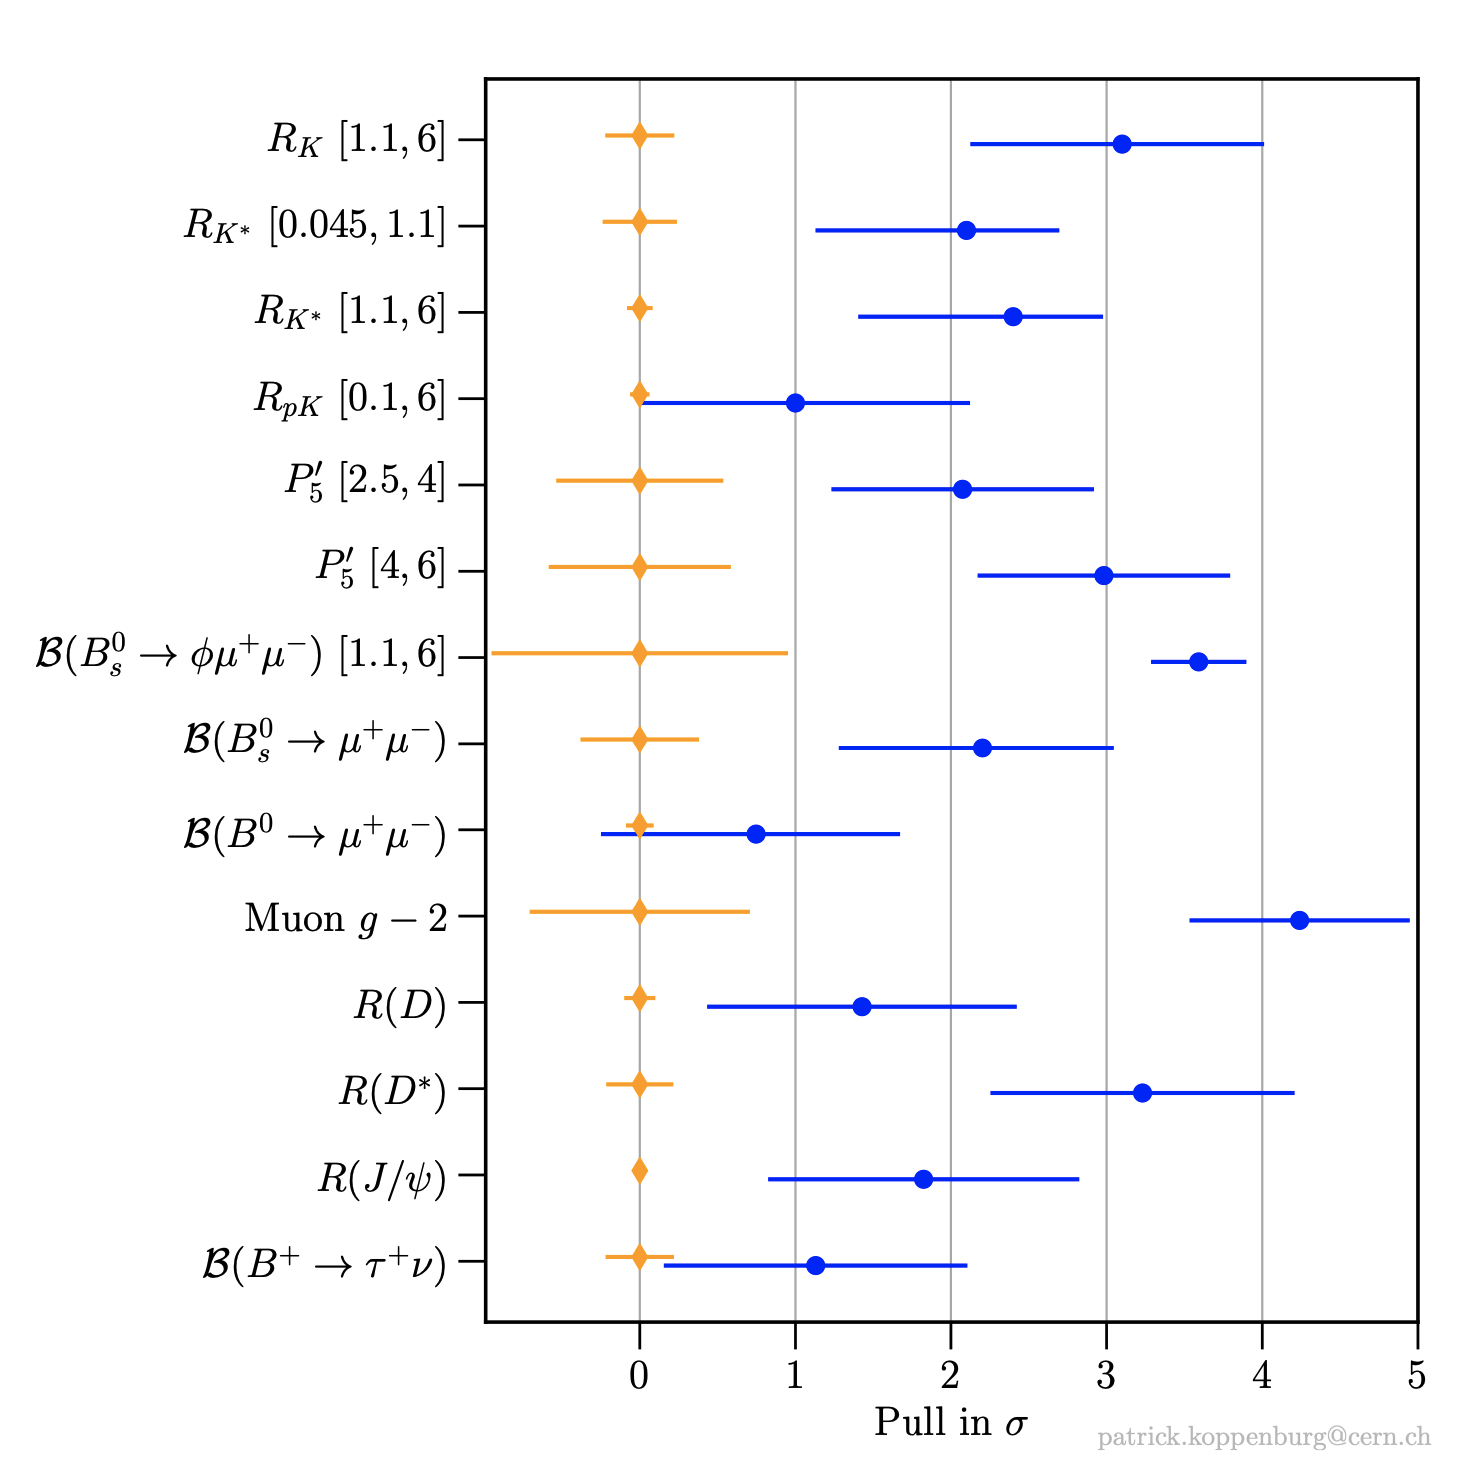
\includegraphics[width=0.65\textwidth]{fig/pull}
	\caption{ Forest plot summarising the flavour observables in tension with the SM predictions, the experimental pull in terms of standard deviations $\sigma$ is shown in blue, while the SM prediction with the theoretical uncertainties is highlighted in orange. This figure is made by P.~Koppenburg~\cite{Koppenburg:2767155}. }
	\label{fig:pull}
\end{figure}
The simultaneous resolution for the anomalies emerging from $ b \to s \ell \ell$ and the semileptonic $b \to c$ transitions, requires models with complicated flavour structure~\cite{DiLuzio:2017vat,Calibbi:2017qbu,Bordone:2017bld,Barbieri:2017tuq,Assad:2017iib,Heeck:2018ntp,Fornal:2018dqn,Crivellin:2018yvo,Crivellin:2019dwb,Bordone:2019uzc}, as such models need to accommodate for similar deviations from the SM for both classes albeit these two transitions occur at different orders in the SM. Such models are often being at the edge of flavour physics constraints~\cite{Bona:2007vi,Silvestrini:2018dos} and collider bounds~\cite{Greljo:2017vvb,Baker:2019sli}.
On the other hand, most up-to-date measurements of $R_{D^{(*)}}$ from the Belle collaboration~\cite{Hirose:2016wfn,Abdesselam:2019dgh} turns out to be in good agreement with the SM~\cite{Bigi:2016mdz,Bernlochner:2017jka,Bigi:2017jbd,Jaiswal:2017rve}, thereby casting some doubt on the potential for NP lurking within $b\to c$ transitions. 
Furthermore, the ratios of branching fractions of decays involving the FCNC $b \to s \ell \ell$ transitions have a much lower dependence on the  non-perturbative QCD effects, that $g-2$, and differential distributions of semileptonic $B$-decays~\cite{Capdevila:2016ivx,Serra:2016ivr,Wehle:2016yoi,Alguero:2019pjc} . Therefore, the LUV information extracted from such ``clean'' observables have the highest potential for extracting LUV insights, see ~\cite{Kou:2018nap} for more details.\\
%%
The  $ b \to s \ell \ell$ anomalies have been studied in a model-independent manner, in particular SMEFT framework in refs.~\cite{DAmico:2017mtc,Geng:2017svp,Capdevila:2017bsm,Ciuchini:2017mik,Hiller:2017bzc} and more recently revisited in refs.~\cite{Ciuchini:2019usw,Aebischer:2019mlg,Alok:2019ufo,Alguero:2019ptt,Kowalska:2019ley,Arbey:2019duh,Datta:2019zca}.  Additionally, many UV-complete models were investigated, particularly leptoquarks~(LQ), like in~refs.~\cite{Calibbi:2015kma,Dorsner:2016wpm,Buttazzo:2017ixm,Kumar:2018kmr,Cornella:2019hct}. Another class of models of special interest are $Z^\prime$ models, in which the $B$ anomalies can be realised at the loop level. The simplest of these models has been proposed in ref.~\cite{Kamenik:2017tnu}, extending the SM with a single new $U(1)$ gauge group, together with the presence of top- and muon-partners, resulting in a top-philic $Z^\prime$ boson capable of evading present collider constraints~\cite{Fox:2018ldq} and responsible for the required LUV signatures. This model has the advantage of not introducing extra flavour spurions to the SM, i.e. similar to the MFV ansatz~\cite{Buras:2000dm,DAmbrosio:2002vsn,Kagan:2009bn}.  A more general set of models with the same features can be found in ref.~\cite{Celis:2017doq} and subsequently elaborated upon in greater detail in the phenomenological study of ref.~\cite{Camargo-Molina:2018cwu}. \\
%%
While evading flavour constraints, models with top-philic $Z^\prime$ are in strong tension with the $Z$-pole measurements~\cite{Camargo-Molina:2018cwu,Efrati:2015eaa}. In fact, it has been shown in~\cite{Ciuchini:2019usw}, that despite large hadronic uncertainties for the amplitude of the $B \to K^{*} \mu^{+} \mu^{-}$ decay, a tension of at the 3$\sigma$ level at least would persist between $B$ data and EWPO for muonic LUV effects, and an even stronger tension would be found in the case of LUV scenarios involving electron couplings. This elucidates the interplay between $B$-physics and EWPO~\cite{Bhattacharya:2014wla,Feruglio:2016gvd,Celis:2017doq,Buttazzo:2017ixm,Kumar:2018kmr,Ciuchini:2019usw,Aebischer:2019mlg,Cornella:2019hct}. \\
%This fact has been brought to light recently~\cite{Coy:2019rfr} to abandon \textit{ii)} and reformulate the original proposal addressing $B$ anomalies at one loop, adding specific {BSM sources of flavour violation to reconcile $B$ data with EW precision tests in this context.} However, as briefly advertised in ref.~\cite{Ciuchini:2019usw}, an important caveat of this EW tension versus $B$ anomalies concerns the assumption of no tree-level NP contributions to EWPO. \\
%#########
This chapter aims to review a global fit, including both EWPO and flavour observables related to the $B$-anomalies. Then present, UV models that accommodate the resulting fit constraints are based on those present in the literature~\cite{Kamenik:2017tnu,Fox:2018ldq,Celis:2017doq},  that accommodate the resulting fit constraints investigated. This work is an extension of several studies done by some of my collaborators~\cite{Ciuchini:2015qxb,Ciuchini:2016weo,Ciuchini:2017mik,Ciuchini:2017gva,Ciuchini:2018xll,Ciuchini:2018anp,Ciuchini:2019usw}, and published in~\cite{Alasfar:2020mne}. 
This chapter is organised as follows: in \autoref{sec:theory}, the SMEFT analysis of the flavour anomalies is presented; in \autoref{sec:UVtoymodels1}, I discuss a viable $Z^{\prime}$ model in relation to our EFT results. After that, I present a possible alternative leptoquark scenarios in~ \autoref{sec:UVtoymodels2}. Lastly, the conclusions are summarised in \autoref{sec:sum}.
%%%%%%%%%%%%%%%%%%
\section{Flavour anomalies in SMEFT }
\label{sec:theory}
%%%%%%%%%%%%%%%%%%
\subsection{Theoretical preamble}
Global fits from $ b \to s \ell \ell$ anomalies show that if the NP degrees of freedom enter at tree-level, they would have an energy scale $ \Lambda \sim 10$ TeV~\cite{DAmico:2017mtc,Geng:2017svp,Capdevila:2017bsm,Ciuchini:2017mik,Hiller:2017bzc}. Highlighting that for LHC phenomenology, the use of SMEFT is justified.  The operators of interest for the explanation of these $B$ anomalies are~\cite{Celis:2017doq,Ciuchini:2019usw,Aebischer:2019mlg}: 
\begin{eqnarray}
	\label{eq:tree_LUV_SMEFT}
	\mathcal{O}_{LQ^{(1)}}^{\ell \ell 23}, \,	(\mathcal{O}_{LQ}^{(1,3)})^{\ell \ell 23}, \, \mathcal{O}_{Qe}^{23 \ell \ell}, \,  \mathcal{O}_{Ld}^{ \ell \ell 23}, \, \mathcal{O}_{ed}^{\ell \ell 23 }.
\end{eqnarray}
Following the same convention for the SM fields, in~\autoref{tab:thesm} and operator definitions in the Warsaw basis are presented in~\autoref{warsaw}.  Current data, taking non-perturbative QCD effects into account using light-cone sum rules, both left- and right-handed operators are permitted ~\cite{Ciuchini:2019usw,Alok:2019ufo,Alguero:2019ptt,Kowalska:2019ley}. Nevertheless, the statistical significance for the right-handed $b \to s$ interaction remains small, coming only from~$R_{K^{*}}/R_{K} \neq 1$ ~\cite{Hiller:2017bzc,Ciuchini:2019usw}. Hence, one can only consider the left-handed operators ~$(	\mathcal{O}_{LQ}^{(1,3)} )^{22 23}$ and~$\mathcal{O}_{Qe}^{23 22}$ for addressing the flavour anomalies. Additionally, when conservative hadronic uncertainties are considered~\cite{Jager:2014rwa,Ciuchini:2015qxb,Arbey:2018ics}, the preference of NP coupling to the muons exclusively becomes mitigated and the inclusion of electron interactions becomes viable as well ~\cite{Ciuchini:2017mik}. From these considerations, we conclude that the operator~$(	\mathcal{O}_{LQ}^{(1,3)} )^{\ell \ell 23}$ with either or both~$ \ell=e, \mu$  offers the minimal resolution of these anomalies within the SMEFT framework~\cite{Ciuchini:2019usw}.\\
Introducing these operators at tree-level will lead to flavour violation beyond the SM, as these operators are flavour spurions unrelated to the SM flavour violation. This can be avoided if they get generated at loop level from the RGE of operators involving the leptons and the Higgs~\cite{Celis:2017doq} 
\begin{eqnarray} 
	\label{eq:SMEFT_op_HL}
	(	\mathcal{O}_{\phi L}^{(1,3)})^{\ell \ell},	\,\,\, 	\mathcal{O}_{\phi e}^{\ell \ell},
\end{eqnarray}
or alternatively, from the semileptonic four-fermion (SL-4F) operators with right-handed top-quark currents:
\begin{eqnarray} 
	\label{eq:SMEFT_op_loop_lu}
	\mathcal{O}_{Lu}^{\ell \ell 3 3}, \,	\,\,	\mathcal{O}_{eu}^{\ell \ell 3 3} 
\end{eqnarray}
The leading log solution of the RGE for these operators ~\cite{Jenkins:2013zja,Jenkins:2013wua}, with the matching conditions for the left-handed quark-current operators in eq.~\eqref{eq:tree_LUV_SMEFT} at the  EW scale $\mu_{\textrm{\tiny{EW}}}\sim v $ are:\footnote{similar to the previous chapters, for one-loop effects,  the NP scale is set to be $\Lambda = 1$~TeV.  The renormalisation scale is set to $\mu_{\rm EW} = m_t\simeq v/\sqrt{2}$ to minimise the matching-scale dependence with the inclusion of the NLO corrections~\cite{Aebischer:2015fzz,Bobeth:2017xry}.}
\begin{eqnarray}
	\label{eq:SMEFT_matching_1loop}
	C_{LQ}^{(1)}\ ^{\ell \ell 23} &=& V_{ts}^{*} V^{ }_{tb} \left(\frac{y_{t} }{4 \pi}\right)^2 \log \left( \frac{\Lambda}{\mu_{\textrm{\tiny{EW}}}} \right)   \, \left(C_{Lu}^{\ell \ell 3 3} - C_{\phi L}^{(1)}\ ^{\ell \ell} \right)\,,\nonumber \\
	C_{LQ}^{(3)}\ ^{\ell \ell 23} &=& V_{ts}^{*} V^{ }_{tb} \left(\frac{y_{t} }{4 \pi}\right)^2 \log \left( \frac{\Lambda}{\mu_{\textrm{\tiny{EW}}}} \right)  \ C_{\phi L}^{(3)}\ ^{\ell \ell}  \,,\nonumber \\
	C_{Qe}^{23\ell \ell} &=& V_{ts}^{*} V^{ }_{tb} \left(\frac{y_{t} }{4 \pi}\right)^2 \log \left( \frac{\Lambda}{\mu_{\textrm{\tiny{EW}}}} \right)   \, \left( C_{eu}^{\ell \ell 3 3} - C^{\ell \ell}_{\phi e}\right) \, .
\end{eqnarray}
%%%%%%
In heavy quark physics, $B$ decays are typically studied within the low energy weak effective theory~\cite{Buchalla:1995vs,Buras:1998raa,Silvestrini:2019sey}, in which we have the vector and axial currents defined as
\begin{eqnarray}
	\label{eq:_Q9_Q10}
	\mathcal{O}_{9 V, \ell} & = & \frac{\alpha_{e}}{8 \pi} (\bar{s} \gamma_{\mu} (1-\gamma_{5})b) ( \bar{\ell} \gamma^{\mu} \ell ) \nonumber \ , \ \\
	\mathcal{O}_{10 A, \ell} & = & \frac{\alpha_{e}}{8 \pi} (\bar{s} \gamma_{\mu} (1-\gamma_{5})b) ( \bar{\ell} \gamma^{\mu} \gamma_{5} \ell ) \ ,
\end{eqnarray}
and matched at the EW scale $\mu_{\textrm{\tiny{EW}}}$  with the SMEFT operators in  eq.~\eqref{eq:SMEFT_op_HL}~-~\eqref{eq:SMEFT_op_loop_lu} follows:
\begin{eqnarray} 
	\label{eq:_C9_C10}
	C_{9,\ell}^{\rm NP}&=& \frac{\pi v^{2}}{\alpha \Lambda^2} \left(\frac{y_{t} }{4 \pi}\right)^2 \log \left( \frac{\Lambda}{\mu_{\textrm{\tiny{EW}}}} \right)   \, \left(C_{\phi L}^{(3)}\ ^{\ell \ell}-C_{\phi L}^{(1)}\ ^{\ell \ell}-C^{\ell \ell}_{\phi e}+ C_{Lu}^{\ell \ell 3 3} + C_{eu}^{\ell \ell 3 3} \right)\,,\nonumber \\
	C_{10,\ell}^{\rm NP}&=& \frac{\pi v^{2}}{\alpha \Lambda^2} \left(\frac{y_{t} }{4 \pi}\right)^2 \log \left( \frac{\Lambda}{\mu_{\textrm{\tiny{EW}}}} \right)   \, \left(C_{\phi L}^{(1)}\ ^{\ell \ell}-C_{\phi L}^{(1)}\ ^{\ell \ell}-C^{\ell \ell}_{\phi e}-s C_{Lu}^{\ell \ell 3 3} + C_{eu}^{\ell \ell 3 3} \right)\, .
\end{eqnarray} 
The overall normalisation in the effective weak Hamiltonian follows the standard conventions adopted in refs.~\cite{Ciuchini:2015qxb,Ciuchini:2017mik,Ciuchini:2019usw}.
%%
As anticipated, the set of operators of interest for the study of $R_{K^{(*)}}$ in eq.~\eqref{eq:SMEFT_matching_1loop} is also sensitive to EWPO.  The operators involving the Higgs field and lepton bilinears in the SMEFT induce tree-level modifications to EW-boson couplings. At the same time, modifications of the $Z$ couplings to the leptons can also be induced via top quark loop
contribution~\cite{deBlas:2015aea}. In the leading-log approximation and at the leading order in the top Yukawa coupling, LUV effects can be generated by:
%
\begin{eqnarray}
	\label{eq:OLuedRGE}
	\left.\Delta g_{Z,L}^{\ell\ell}\right|_{\mathrm{LUV}} & = &
	- \frac 12 \left( C_{\phi L}^{(1)}\ ^{\ell \ell} +C_{\phi L}^{(3)}\ ^{\ell \ell} \right)\frac{v^2}{\Lambda^2}-
	3 \left( \frac{ y_t \, v}{4 \pi \Lambda} \right)^2 \log\left(\frac{\Lambda}{\mu_{\textrm{\tiny{EW}}}} \right) \, C_{Lu}^{\ell\ell33}  \ , \\ \nonumber
	\left.\Delta g_{Z,R}^{\ell\ell}\right|_{\mathrm{LUV}} & = & 
	- \frac 12 C^{\ell\ell}_{\phi e}\frac{v^2}{\Lambda^2}-
	3 \left( \frac{ y_t \, v}{4 \pi \Lambda} \right)^2 \log\left(\frac{\Lambda }{\mu_{\textrm{\tiny{EW}}}}\right) \, C_{eu}^{\ell\ell33} \ ,
\end{eqnarray}
where $\Delta g_{Z,L (R)}^{\ell\ell} \equiv g_{Z,L(R)}^{\ell\ell} - g_{Z,L (R)}^{\ell\ell,\textrm{SM}}$ is the deviation with respect to the left-handed (right-handed) leptonic couplings to the $Z$ boson in the SM theory. Since EW couplings to leptons have been precisely measured at LEP/SLC, they provide an important test threshold for lepton universality~\cite{Efrati:2015eaa,deBlas:2016ojx}.\\

These observations motivate a global SMEFT fit of the operators explaining the  $B$-anomalies and their interplay with EWPO.  Assuming that the LUV effects are generated by NP via radiative effects, matching what is seen in eq.~(\ref{eq:_C9_C10}). Consequently, the NP will contribute to EWPO at the tree level, whilst other SMEFT operators from the REG mixing are assumed to be small or constrained from other processes.  For these assumptions to be fulfilled within SMEFT, the operators modifying the EW coupling of the quarks need to be included as well 
\begin{eqnarray} 
	\label{eq:SMEFT_op_HQ}
	\mathcal{O}_{\phi Q}^{(1)} \ ^{qq} , \,
	\mathcal{O}_{\phi Q}^{(3)}\ ^{qq} ,\,  
	\mathcal{O}_{\phi u}^{qq}, \, 
	\mathcal{O}_{\phi d}^{qq}, 
\end{eqnarray}
where $q=1,2,3$ identifies quark generations. These operators are considered to be flavour aligned, in a similar fashion to $C_{q\phi}$ of the previous chapter; in particular, they are assumed to be aligned with the down-quark basis. This is needed to avoid pathological tree-level FCNC ~\cite{Silvestrini:2018dos}. The same holds for the leptonic operators, aligned with the charged lepton mass bases.\\
%
The EWPO have a degeneracy between the first and second-generation quarks, particularly in the down-type quarks sector. Therefore, it is natural to impose a $U(2)^3$ symmetry between first and second generator quark operators, thus imposing $C_{\phi Q}^{(1,3)}\ ^{11} = C_{\phi Q}^{(1,3)}\ ^{22} $, $C_{\phi u}^{11} = C_{\phi u}^{22}$. This also helps to suppress large FCNC contributions from these operators.  Additionally, the RGE boundary condition $C^{33}_{\phi u}=0$ is assumed. This is motivated by the fact that this Wilson coefficient cannot be constrained by EWPO, as modifications to $Z$-coupling to right-handed top quarks cannot be probed by $Z$-pole measurements. 
Finally, for completeness, the four-lepton operator is also included in the fit:
\begin{equation}
	\label{eq:SMEFT_op_LLLL}
	O^{1221}_{LL}=(\bar{L}_1 \gamma^\mu L_2) (\bar{L}_2 \gamma_\mu L_1) \ ,
\end{equation}
which contributes to the muon decay amplitude, and therefore alters the extraction of the value of the Fermi constant, $G_F$, which is one of the inputs of the SM EW sector.

The operators in eqs.~\eqref{eq:SMEFT_op_HL}, \eqref{eq:SMEFT_op_HQ} and \eqref{eq:SMEFT_op_LLLL}, with the assumptions mentioned before, saturate all the 17 degrees of freedom, i.e. combinations of operators, that can be constrained in a fit to EWPO in the dimension-six SMEFT framework while keeping flavour changing neutral currents in the light quark sector under control. Together with the 4 four-fermion operators from eq.~\eqref{eq:SMEFT_op_loop_lu}, this completes a total of 21 operators, which is included in the fit setup described in the next section. 
%%%%%%%%%%%%%%%%%%
\subsection{SMEFT fit}
\label{sec:strategy}
%%%%%%%%%%%%%%%%%%
The global fit combining both flavour observables related to the $ b \to s \ell \ell$ anomalies and EWPO is carried out in a Bayesian statistical framework. The experimental observables are modelled via state-of-the-art theoretical information already implemented and described in ref.~\cite{Ciuchini:2019usw} for flavour physics and EW and Higgs physics in ref.~\cite{Ciuchini:2013pca} and, more recently, in ref.~\cite{deBlas:2016ojx}. EWPO are extended by flavour non-universal  SMEFT contributions described in ref.~\cite{Efrati:2015eaa,deBlas:2019wgy}. The statistical and physics frameworks are available within the publicly available \HEPfit~\cite{deBlas:2019okz} package. An MCMC framework built using the Bayesian Analysis Toolkit~\cite{2009CoPhC.180.2197C}~\footnote{ \HEPfit is developed by some of my collaborators, who have co-authored this work}\\
The experimental input used for the global is summarised in the following, which are also implemented in \HEPfit code: 
\begin{itemize}
	\setlength\itemsep{0em}
	{\item The set of EWPO including the $Z$-pole and $W$ properties measurements from LEP and SLD, in addition to  Tevatron and LHC measurements of  EW bosons properties and rates ~\cite{ALEPH:2005ab,Abe:2000uc,Group:2012gb,Schael:2013ita,Aaboud:2017svj,Khachatryan:2014iya,Abazov:2011ws}. The following EWPO used in the fit are
		%
		\begin{gather*}
			M_H,~m_t,~\alpha_S(M_Z),~\Delta \alpha_{\mathrm{had}}^{(5)}(M_Z),\\
			M_{Z},~\Gamma_{Z},~R_{e,\mu,\tau},~\sigma_{\mathrm{had}}, ~A^{e,\mu,\tau}_{FB},~A_{e,\mu,\tau},~A_{e,\tau}(P_\tau),~ R_{c,b},~A^{c,b}_{FB},~A_{s,c,b},~R_{u+c}, \\
			M_{W},\Gamma_{W},~\mathrm{BR}_{W\to e \nu,\mu \nu,\tau \nu},~\Gamma_{W\to cs}/\Gamma_{W\to ud+cs},~\left|V_{tb}\right|;
		\end{gather*}
		%
	}
	\item The angular distribution of the decay $B\to K^{(*)}\ell^+\ell^-$ including both the$\mu$ and $e$ final states in the large $m_{\ell \ell}$ bins~\footnote{The measurements of  $B\to K^{(*)}\ell^+\ell^-$ decays in the low di-lepton invariant mass region are plagued by large uncertainties for the $J/\psi$ resonance, and thus not included in the fit.}.   The data from ATLAS~\cite{Aaboud:2018krd}, Belle~\cite{Wehle:2016yoi}, CMS~\cite{Khachatryan:2015isa,Sirunyan:2017dhj} and LHCb~\cite{Aaij:2015dea,Aaij:2020nrf}, in addition to the branching fractions from LHCb~\cite{Aaij:2016flj}, the charged $B^+$ meson measured by LHCb~\cite{Aaij:2014pli}, and the HFLAV average~\cite{Amhis:2019ckw} for the branching fraction of the decay~$B\to K^*\gamma$; 
	\item The angular distribution of $B_s\to \phi\mu^+\mu^-$~\cite{Aaij:2015esa} and the branching ratio of  the decay $B_s\to\phi\gamma$~\cite{Aaij:2012ita}, measured by LHCb;
	\item The LUV ratios $R_K$~\cite{Aaij:2019wad} and $R_{K^*}$~\cite{Aaij:2017vbb} from LHCb and Belle~\cite{Abdesselam:2019wac};
	\item Branching ratio of $B_{(s)}\to \mu^+\mu^-$ measured by LHCb~\cite{Aaij:2017vad}, CMS~\cite{Chatrchyan:2013bka}, and ATLAS~\cite{Aaboud:2018mst}; in addition to the upper bound on the decay $B_s\to e^+e^-$ reported by LHCb~\cite{Aaij:2020nol}. 
\end{itemize}
Modelling the decays of hadrons involves factorisable (in terms of the decay constant) and non-factorisable non-perturbative QCD effects. The non-factorisable effects emerge from long-distance hadronic contributions to~\cite{Khodjamirian:2010vf,Jager:2014rwa,Lyon:2014hpa} QCD loops appearing in radiative corrections to these decays. In this analysis, the ~$B\to K^*\ell^+\ell^-$ has two different scenarios to describe these hadronic effects, also discussed in other previous works of my collaborators ~\cite{Ciuchini:2016weo,Ciuchini:2017mik,Ciuchini:2017gva,Ciuchini:2018xll,Ciuchini:2018anp, Ciuchini:2019usw}. The first is a conservative approach (Phenomenological Data-Driven or PDD) as originally proposed in \cite{Ciuchini:2015qxb}, and refined in ref.~\cite{Ciuchini:2018anp}, whilst the second is a more optimistic one based on the results in~\cite{Khodjamirian:2010vf} (Phenomenological Model Driven or PMD). The PDD scenario is based on a generic model of the hadronic effects, which is simultaneously fitted to $b \to s \ell \ell$ data alongside the NP effects. Contrary to the PDD approach, in the PMD scenario, the dispersion relations specified in~\cite{Khodjamirian:2010vf} are used to constrain the hadronic contributions in the entire large-recoil region considered in the analysis. Ergo, PMD has smaller hadronic effects in the~$B\to K^*\ell^+\ell^-$ amplitudes~\cite{Ciuchini:2016weo}. The choice of the hadronic uncertainties model significantly affects the outcome of the fits to the $B$-decays observables~\cite{Ciuchini:2019usw}. \\ In order to be as general as possible, the SMEFT global fit is done for four different scenarios, described as follows:
\begin{itemize}
	\setlength\itemsep{0em}
	\item {\bf EW}: 
	Using EWPO data only with the assumptions discussed in~\autoref{sec:theory}. This fit includes the operators in eqs.~\eqref{eq:SMEFT_op_HL},~\eqref{eq:SMEFT_op_HQ}, and \eqref{eq:SMEFT_op_LLLL},  giving a total of 17 Wilson coefficients.
	%
	\item  {\bf EW (SL-4F Only)}: This refers to a fit done with the Wilson coefficients of the { SL-4F operators} involving the right-handed top current, reported in eq.~\eqref{eq:SMEFT_op_loop_lu}. This scenario assumes that BSM enters the modifications of the $Z$ couplings to muons and electrons through top-quark loops only.
	%
	\item {\bf EW \& Flavour}: Wilson coefficients of all the { 21 operators} given in eq.~\eqref{eq:SMEFT_op_HL},~\eqref{eq:SMEFT_op_HQ}, and eq.~\eqref{eq:SMEFT_op_LLLL}, together with eq.~\eqref{eq:SMEFT_op_loop_lu} are varied.\\
	All of the EW data and the flavour observables listed above are used. As explained above, this scenario comes in two varieties, PDD and PMD.
	\item {\bf Flavour}: These fits exclusively include the Wilson coefficients of the {\em 4 operators} (both electrons and muons) appearing in eq.~\eqref{eq:SMEFT_op_loop_lu}, and are done including only flavour data, i.e. excluding EW measurements. Results are again distinguished for the PDD and PMD cases. This fit is typically done when flavour anomalies are discussed in the literature. Hence, it was included here to emphasise the importance of including EWPO.
\end{itemize}
%%%%%%%%%%%%%%%%%%
\subsection{Fit results}
\label{sec:EFT_results}
%%%%%%%%%%%%%%%%%%
The fit was performed for each of the aforementioned scenarios, and the extracted average values of the Wilson coefficients and the corresponding 68\% CI are summarised in ~\autoref{fig:ew_flav_bounds}.\\ The EW only fits, involving 17 out of the total 21 Wilson coefficients are shown in~\textcolor[HTML]{be3d04}{orange}. The EWPO fit shows good agreements with the SM within~$2\sigma$ level. Additionally, the Wilson coefficients involved in the fit seem to be highly correlated with the EWPO data as indicated by the correlation matrix in~\autoref{fig:ew_corr}. \\
The impact of these operators on the $ b \to s \ell \ell$ observables are shown in~\autoref{fig:ew_flav_dg}, where  it collects the mean and standard deviation on the shift in the $Z$ coupling to light leptons w.r.t the SM, it should be noted that these deviations of the $Z$ couplings are related to the LUV ratios   $R_{K^{(*)}}$ in the dilepton-mass range $[1.0,6.0]$~GeV$^2$ by: 
\begin{equation}
	\label{eq:SMdev}
	\delta g_{Z,L(R)}^{ee(\mu\mu)} \equiv g_{Z,L(R)}^{ee(\mu\mu)}{\big/}g_{Z,L(R)}^{ee(\mu\mu),\textrm{\tiny SM}}-1  \ , \ \delta R_{K^{(*)}} \equiv R_{K^{(*)}}^{ } - R_{K^{(*)}}^{\textrm{\tiny SM}} \ ,
\end{equation}
which is tightly constraint by the EWPO data to per-mille level. \\
The other fit scenario only involves the \textbf{ SL-4F} coefficients constraint from EWPO data, shown in \textcolor[HTML]{c2b109}{yellow}  in~\autoref{fig:ew_flav_bounds}. Although EW data allows for more relaxed constraints on these operators, for example $\mathcal{O}_{Lu}^{\ell \ell 33}$ compared to the ones modifying $Z$ couplings at tree-level e.g. $\mathcal{O}_{\phi L}$, the bounds remain compatible with the null (SM) Hypothesis and in about $3\sigma$ conflict with the experimental measurements on~$R_{K^{(*)}}$  (indicated by the shaded red boxes in the right side of~\autoref{fig:ew_flav_dg}).  
\\
We now move to the flavour data fits, with both ans\"atze for the hadronic contributions PDD highlighted in~\textcolor[HTML]{0843a5}{blue} and PMD in~ \textcolor[HTML]{c00054}{pink}. For this fit, deviations of the muonic ~$C_{Lu}^{22 33}$ show deviation from the SM hypothesis of $3\sigma$ for PDD and up to $6\sigma$ for the optimistic PMD scenario. The difference in the significance between the two cases stems from the interpretation of the angular analysis --namely the $P^\prime_5$ observable-- of the $B \to K^{*} \mu \mu$ decay. The PDD approach favours the fully left-handed NP coupling, i.e.  $C_{9, \ell} = - C_{10, \ell}$, and allows for NP coupling to electrons, while the PMD exclusively predicts the muonic resolution~\cite{Ciuchini:2017mik,Ciuchini:2019usw}.\\ Flavour data seem to predict deviations in the $Z$ coupling modifiers, implying a tension between the flavour fits and EWPO exacerbated by the PMD modelling of the long-distance QCD effects.  This tension between $B$- anomalies and EW data reach 3(6)$\sigma$ level for PDD(PMD). Of course, introducing a tree-level resolution of the $b \to s \ell \ell$ anomalies would decouple EW sensitive SMEFT operators from the four-fermion operators required for these anomalies. Still, it will not be compatible with the MFV ansatz. In fact, the size of flavour violation introduced by the tree-level resolution of the $B$ anomalies brings any model with such structure to the brick of exclusion by other flavour observables ~\cite{Bona:2007vi,Silvestrini:2018dos,Greljo:2017vvb,Baker:2019sli}.
\\
\begin{sidewaysfigure}[ht]
	\centering
	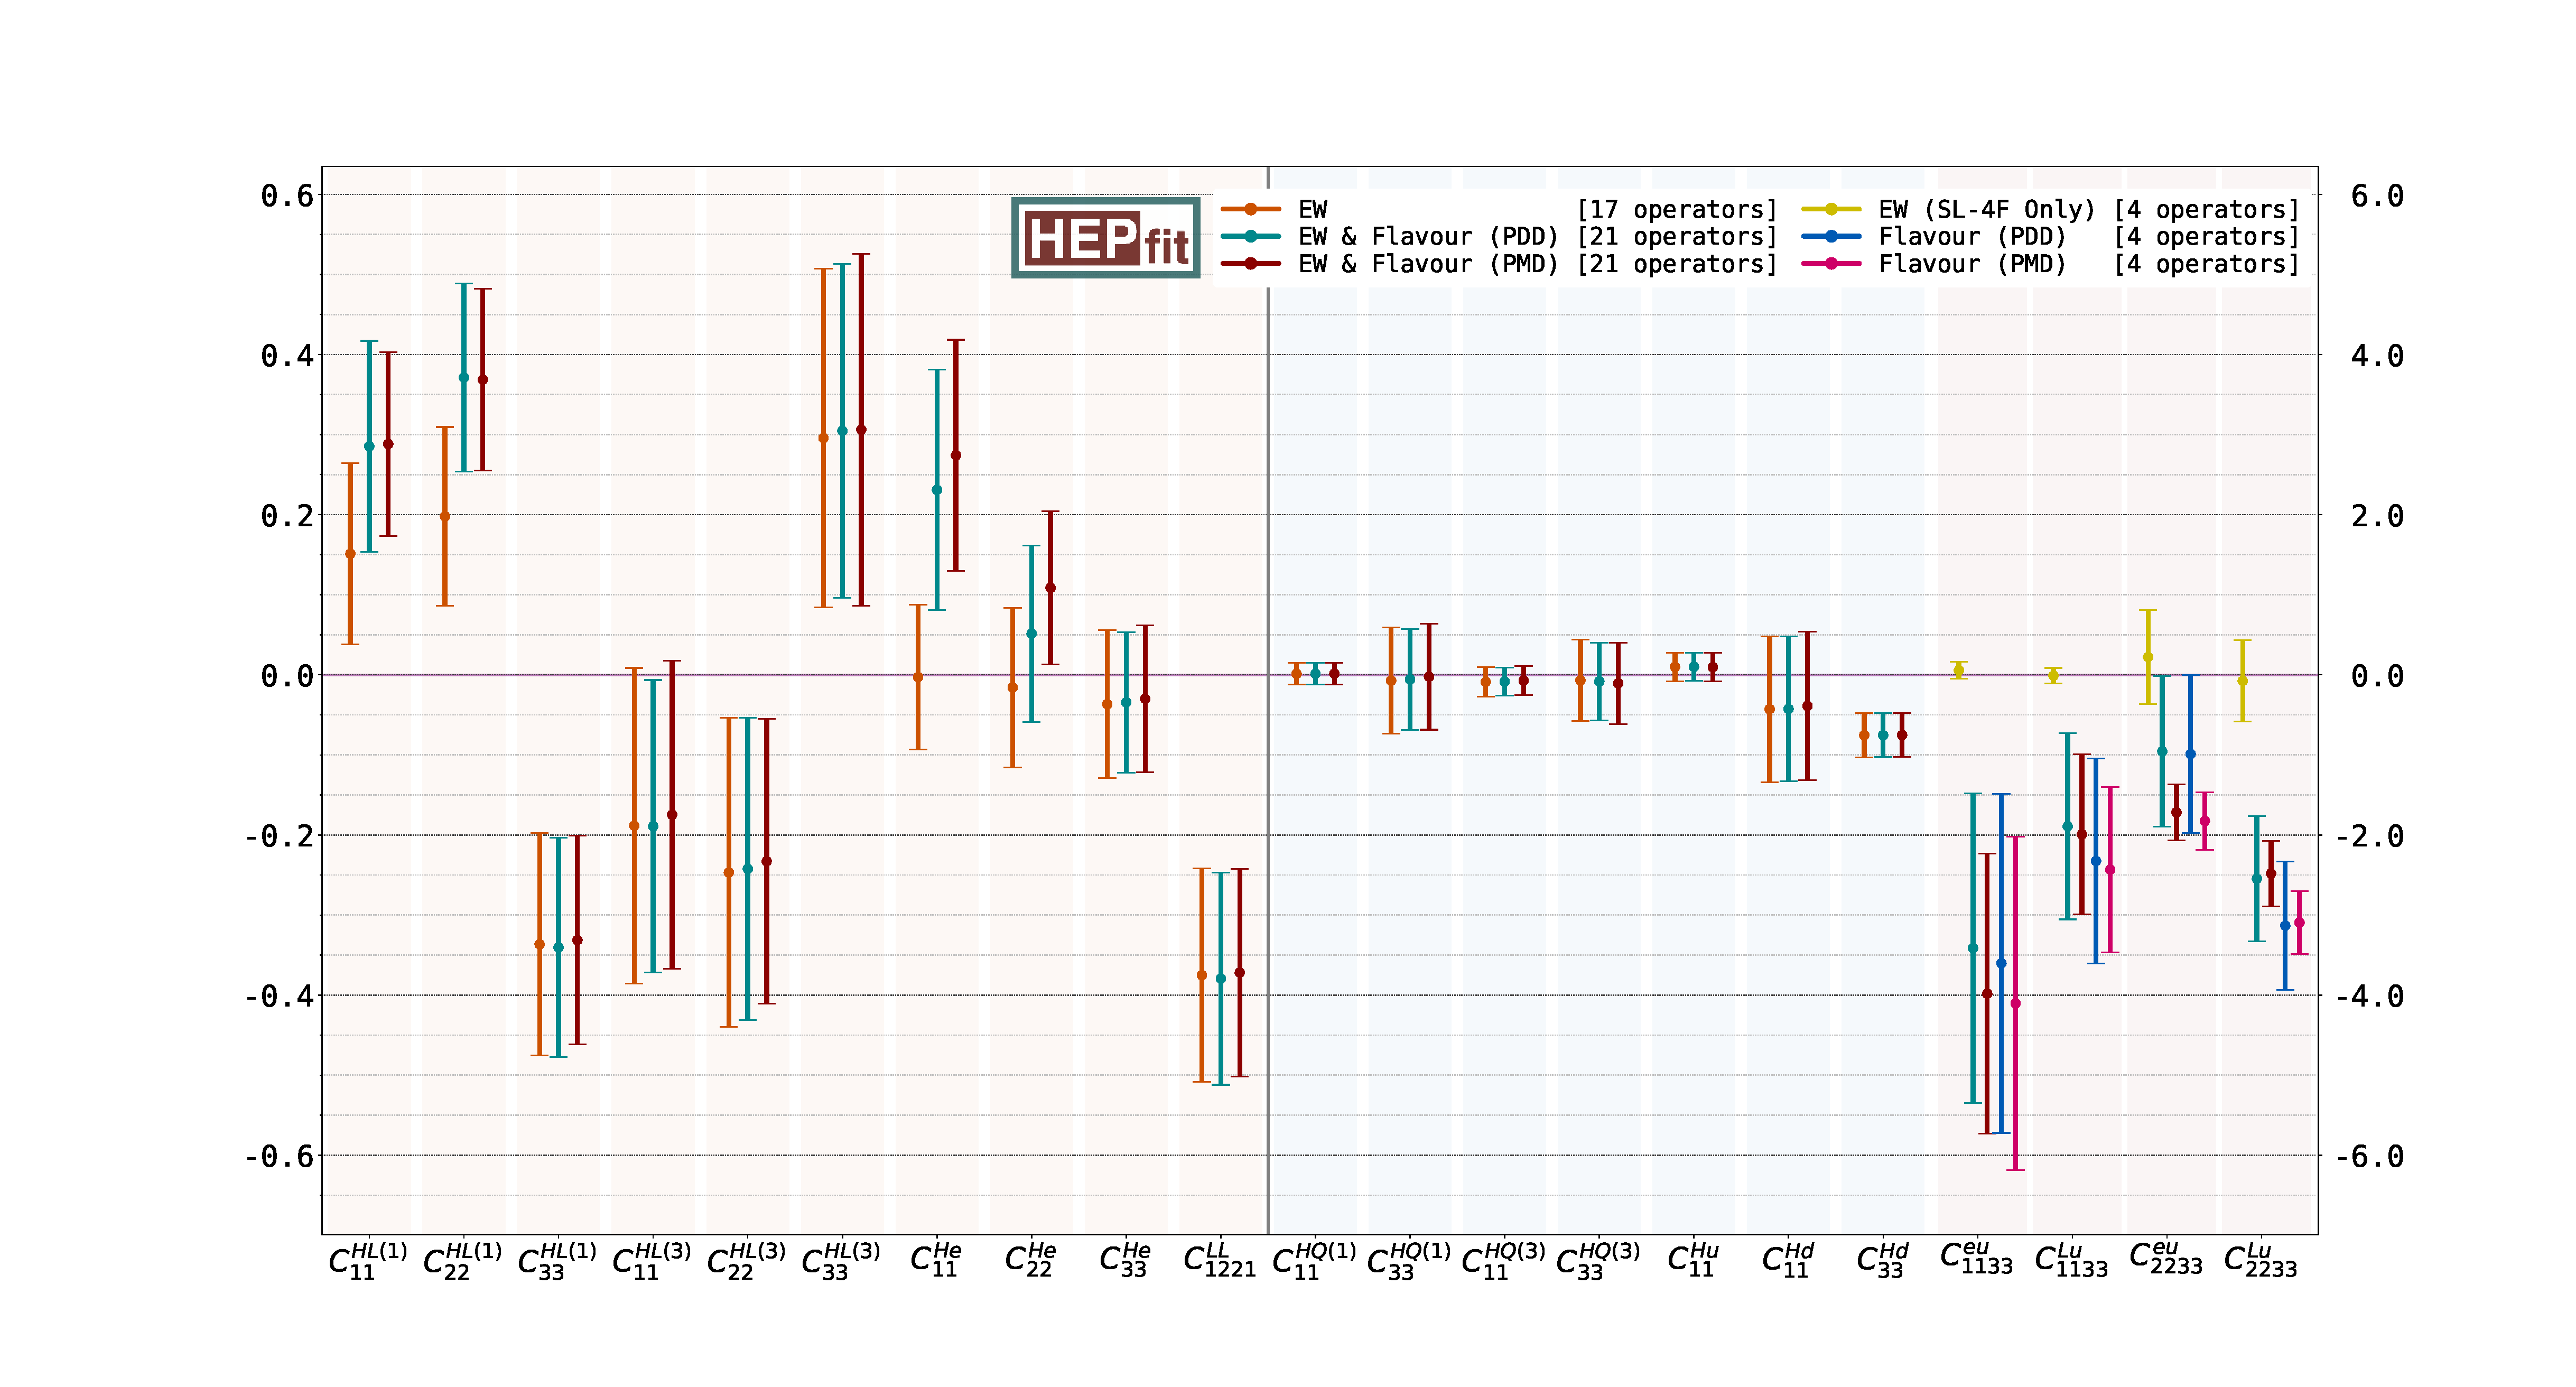
\includegraphics[width=\textwidth]{figures/errorbar.pdf}
	\caption{
		The marginalised fit results of the Wilson coefficients are considered in the scenarios detailed in~\autoref{sec:strategy}. The central points denote the mean of the marginalised posterior distribution, while the error bars are the 68\% CI constraint of the Wilson coefficients.  (Note the different scaling in the axes quantifying the size of the bounds presented in each half of the figure.) This figure is published in~\cite{Alasfar:2020mne}. 
	}
	\label{fig:ew_flav_bounds}
\end{sidewaysfigure}
\FloatBarrier
\begin{figure}[ht!]
	\centering
	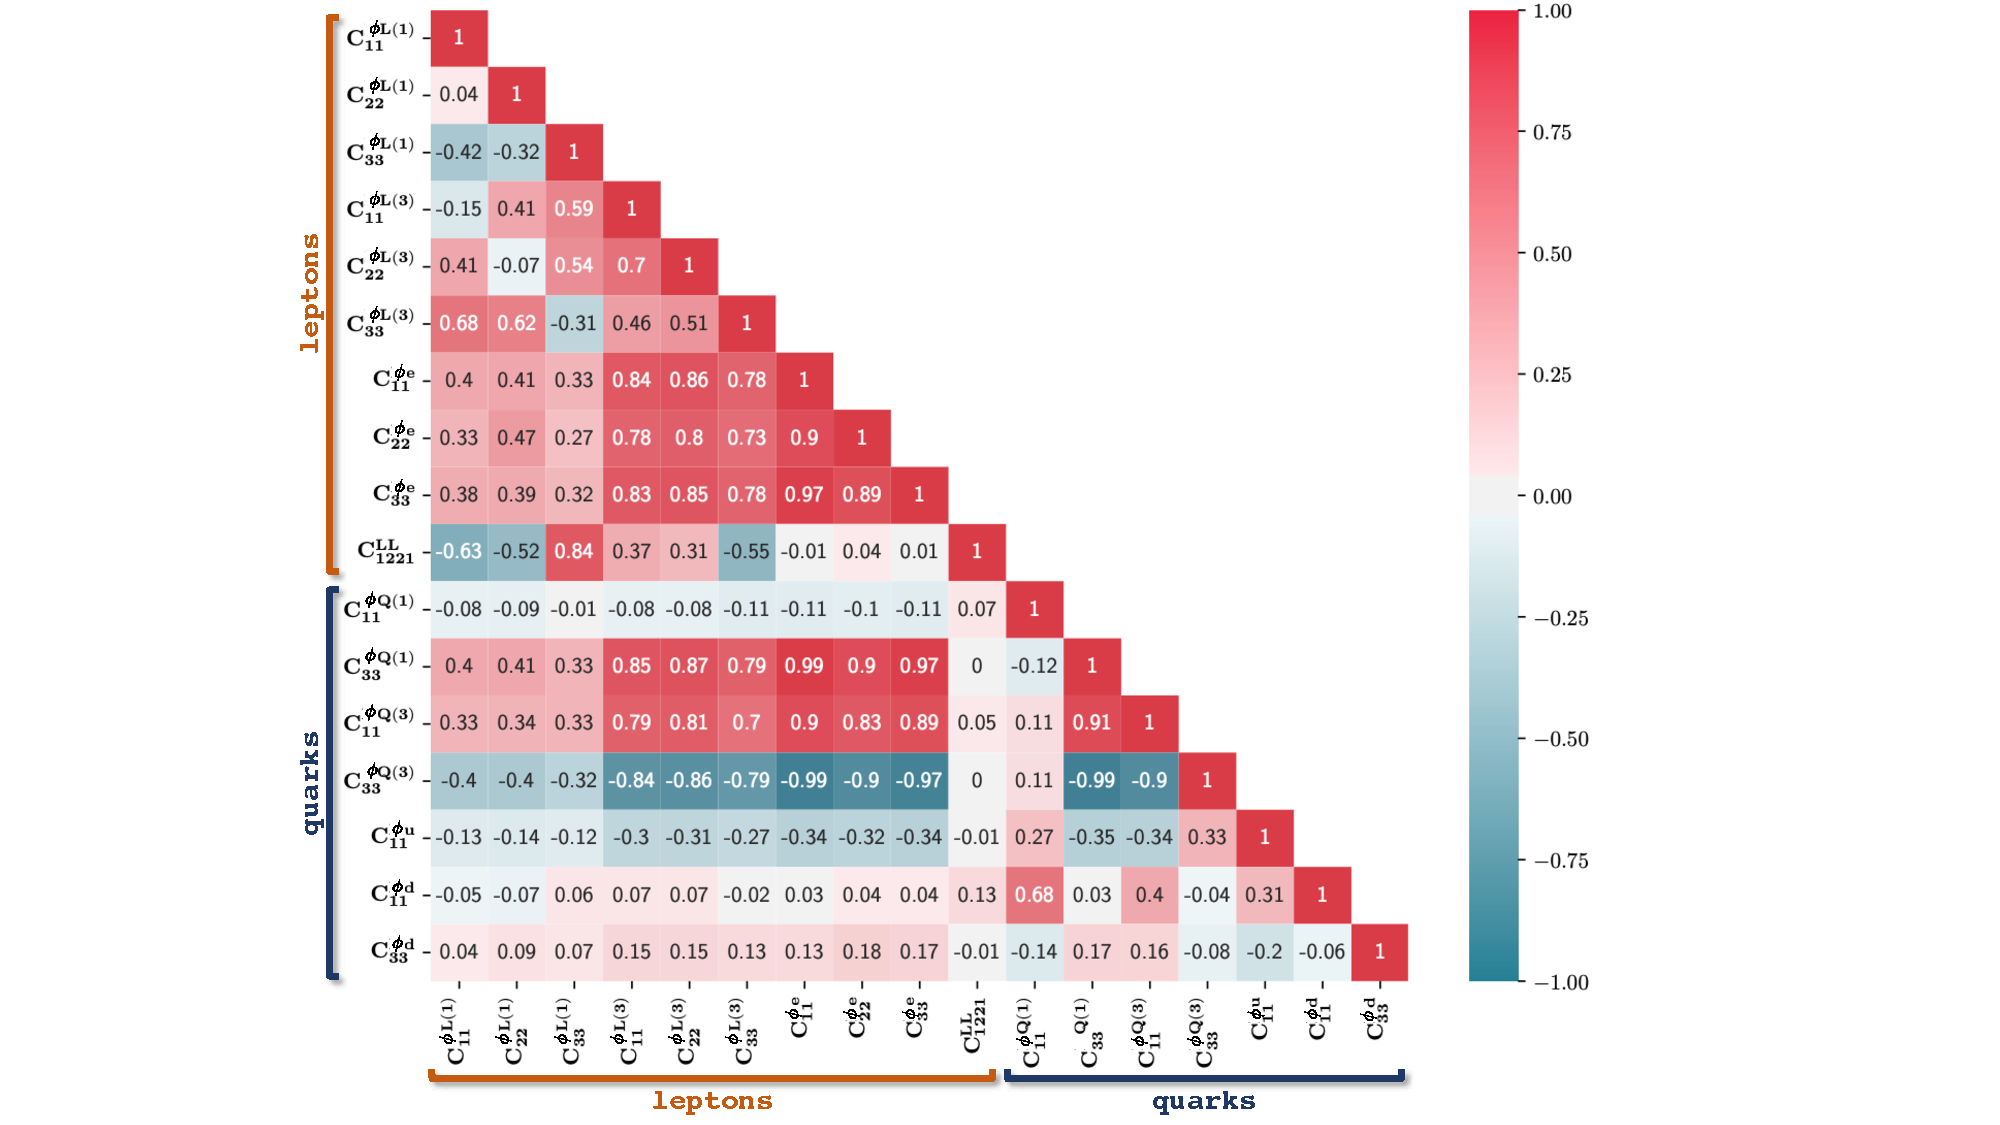
\includegraphics[width=\textwidth]{figures/heatmap_EW_loop.pdf}
	\caption{ The correlation matrix resulting from the Bayesian fit of the Wilson coefficient of the operators listed in in eqs.~\eqref{eq:SMEFT_op_HL}, \eqref{eq:SMEFT_op_HQ}, \eqref{eq:SMEFT_op_LLLL} in the \textbf{EW} scenario introduced in \autoref{sec:strategy}. The two distinct groups of Wilson coefficients associated to leptonic and quark interactions are remarked as ``leptons'' and ``quarks'', respectively. This figure is published in~\cite{Alasfar:2020mne}. }
	\label{fig:ew_corr}
\end{figure}
\begin{figure}[htp!]
	\centering
	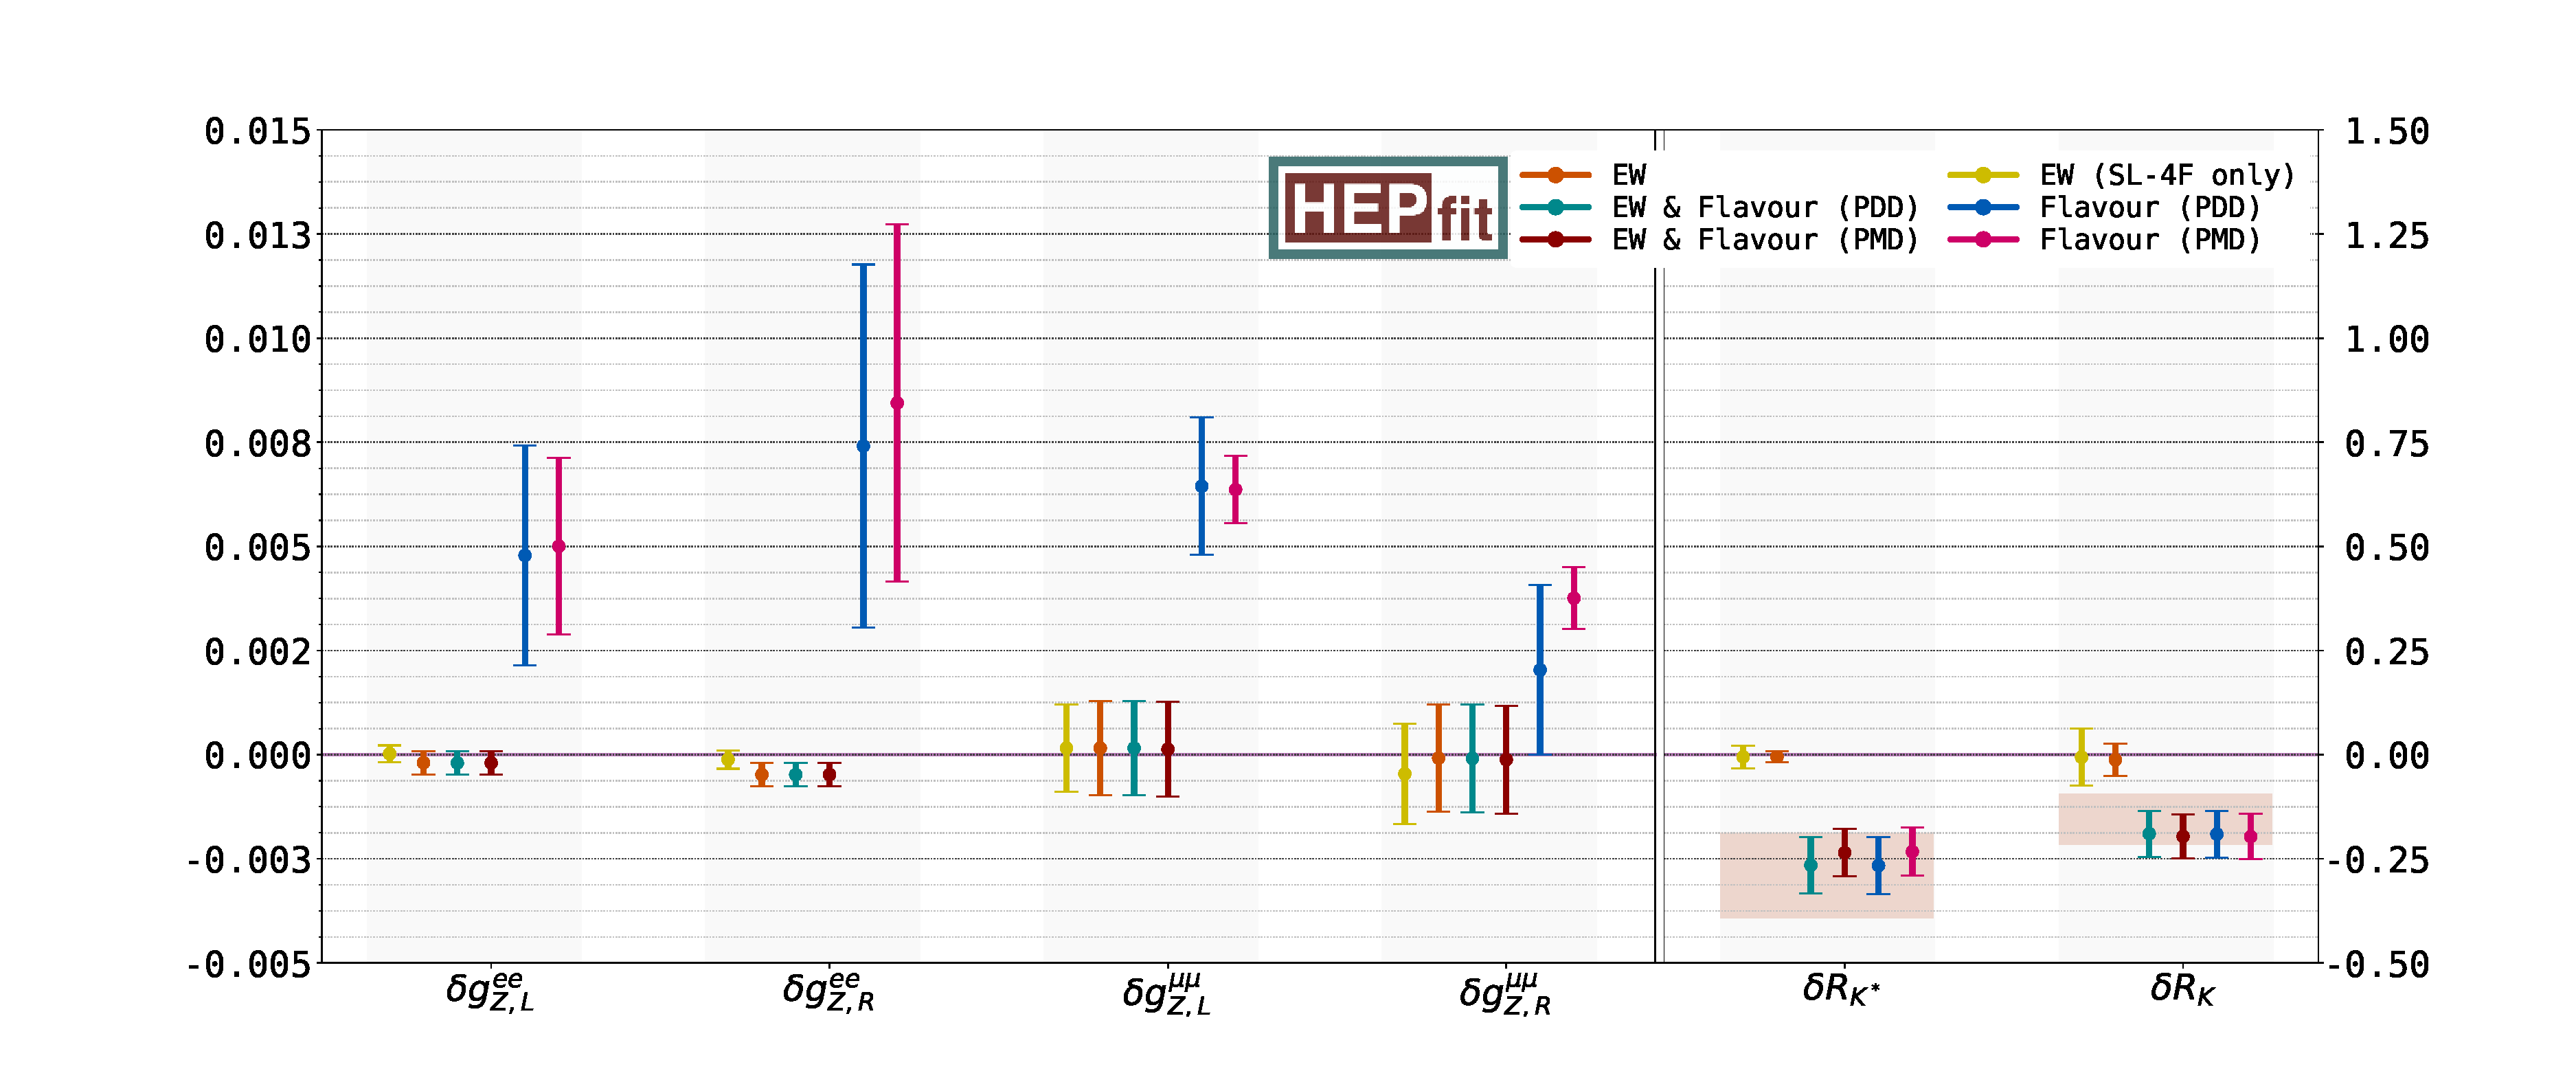
\includegraphics[width=\textwidth]{figures/errorbar_dg.pdf}
	\caption{ Fit results following the same convention as~\autoref{fig:ew_flav_bounds} for the $Z$ boson coupling modifiers for the muons and electrons, as well as the  lepton universality violating ratios, see eq.~\eqref{eq:SMdev}, with the red boxes indicating the region selected by the experimental measurements of $R_{K,(K^*)}$. This figure is published in~\cite{Alasfar:2020mne}. 
	}
	\label{fig:ew_flav_dg}
\end{figure}
A global fit with the 21 coefficients, combining both flavour and EW data, is the way to reach a consensus between what is required by $ b \to e \ell \ell$ observations resolution and EW precision tests. Similarly to the flavour scenario, the fits is preformed for PDD in \textcolor[HTML]{0f7678}{teal}  and PMD in \textcolor[HTML]{760003}{red} in~\autoref{fig:ew_flav_bounds} and \autoref{fig:ew_flav_dg}. In these scenarios, the tension between EWPO and flavour data is lifted as the deviation from the SM $Z$-couplings remains within the EW data predictions. Also, the LUV generated by the Wilson coefficients matches the experimental observations. The resolution comes from deviation of $C_{\phi L (e)}^{\ell \ell}$ and the 4F operators $\mathcal{O}_{(L)eu}^{\ell \ell 3 3}$ from the SM hypothesis. \\ Another interesting observation from the global fit can be seen in the network graphs in~\cite{fig:ew_flav_corr}, wherein the EW only fits the SL-4F Wilson coefficients are degenerate with the Higgs-lepton bilinear currents $C_{\phi L (e)}^{\ell \ell}$, having Pearson's correlation of  $\rho \sim -1.0$. This degeneracy is broken once both EW and flavour data are taken into account, as seen in the lower panels of this figure. The breaking of the degeneracy is the reason for the observed shifts in the posterior distributions of $C_{\phi L (e)}^{\ell \ell}$ from the SM hypothesis. \\
\begin{figure}[h!]
	\centering
	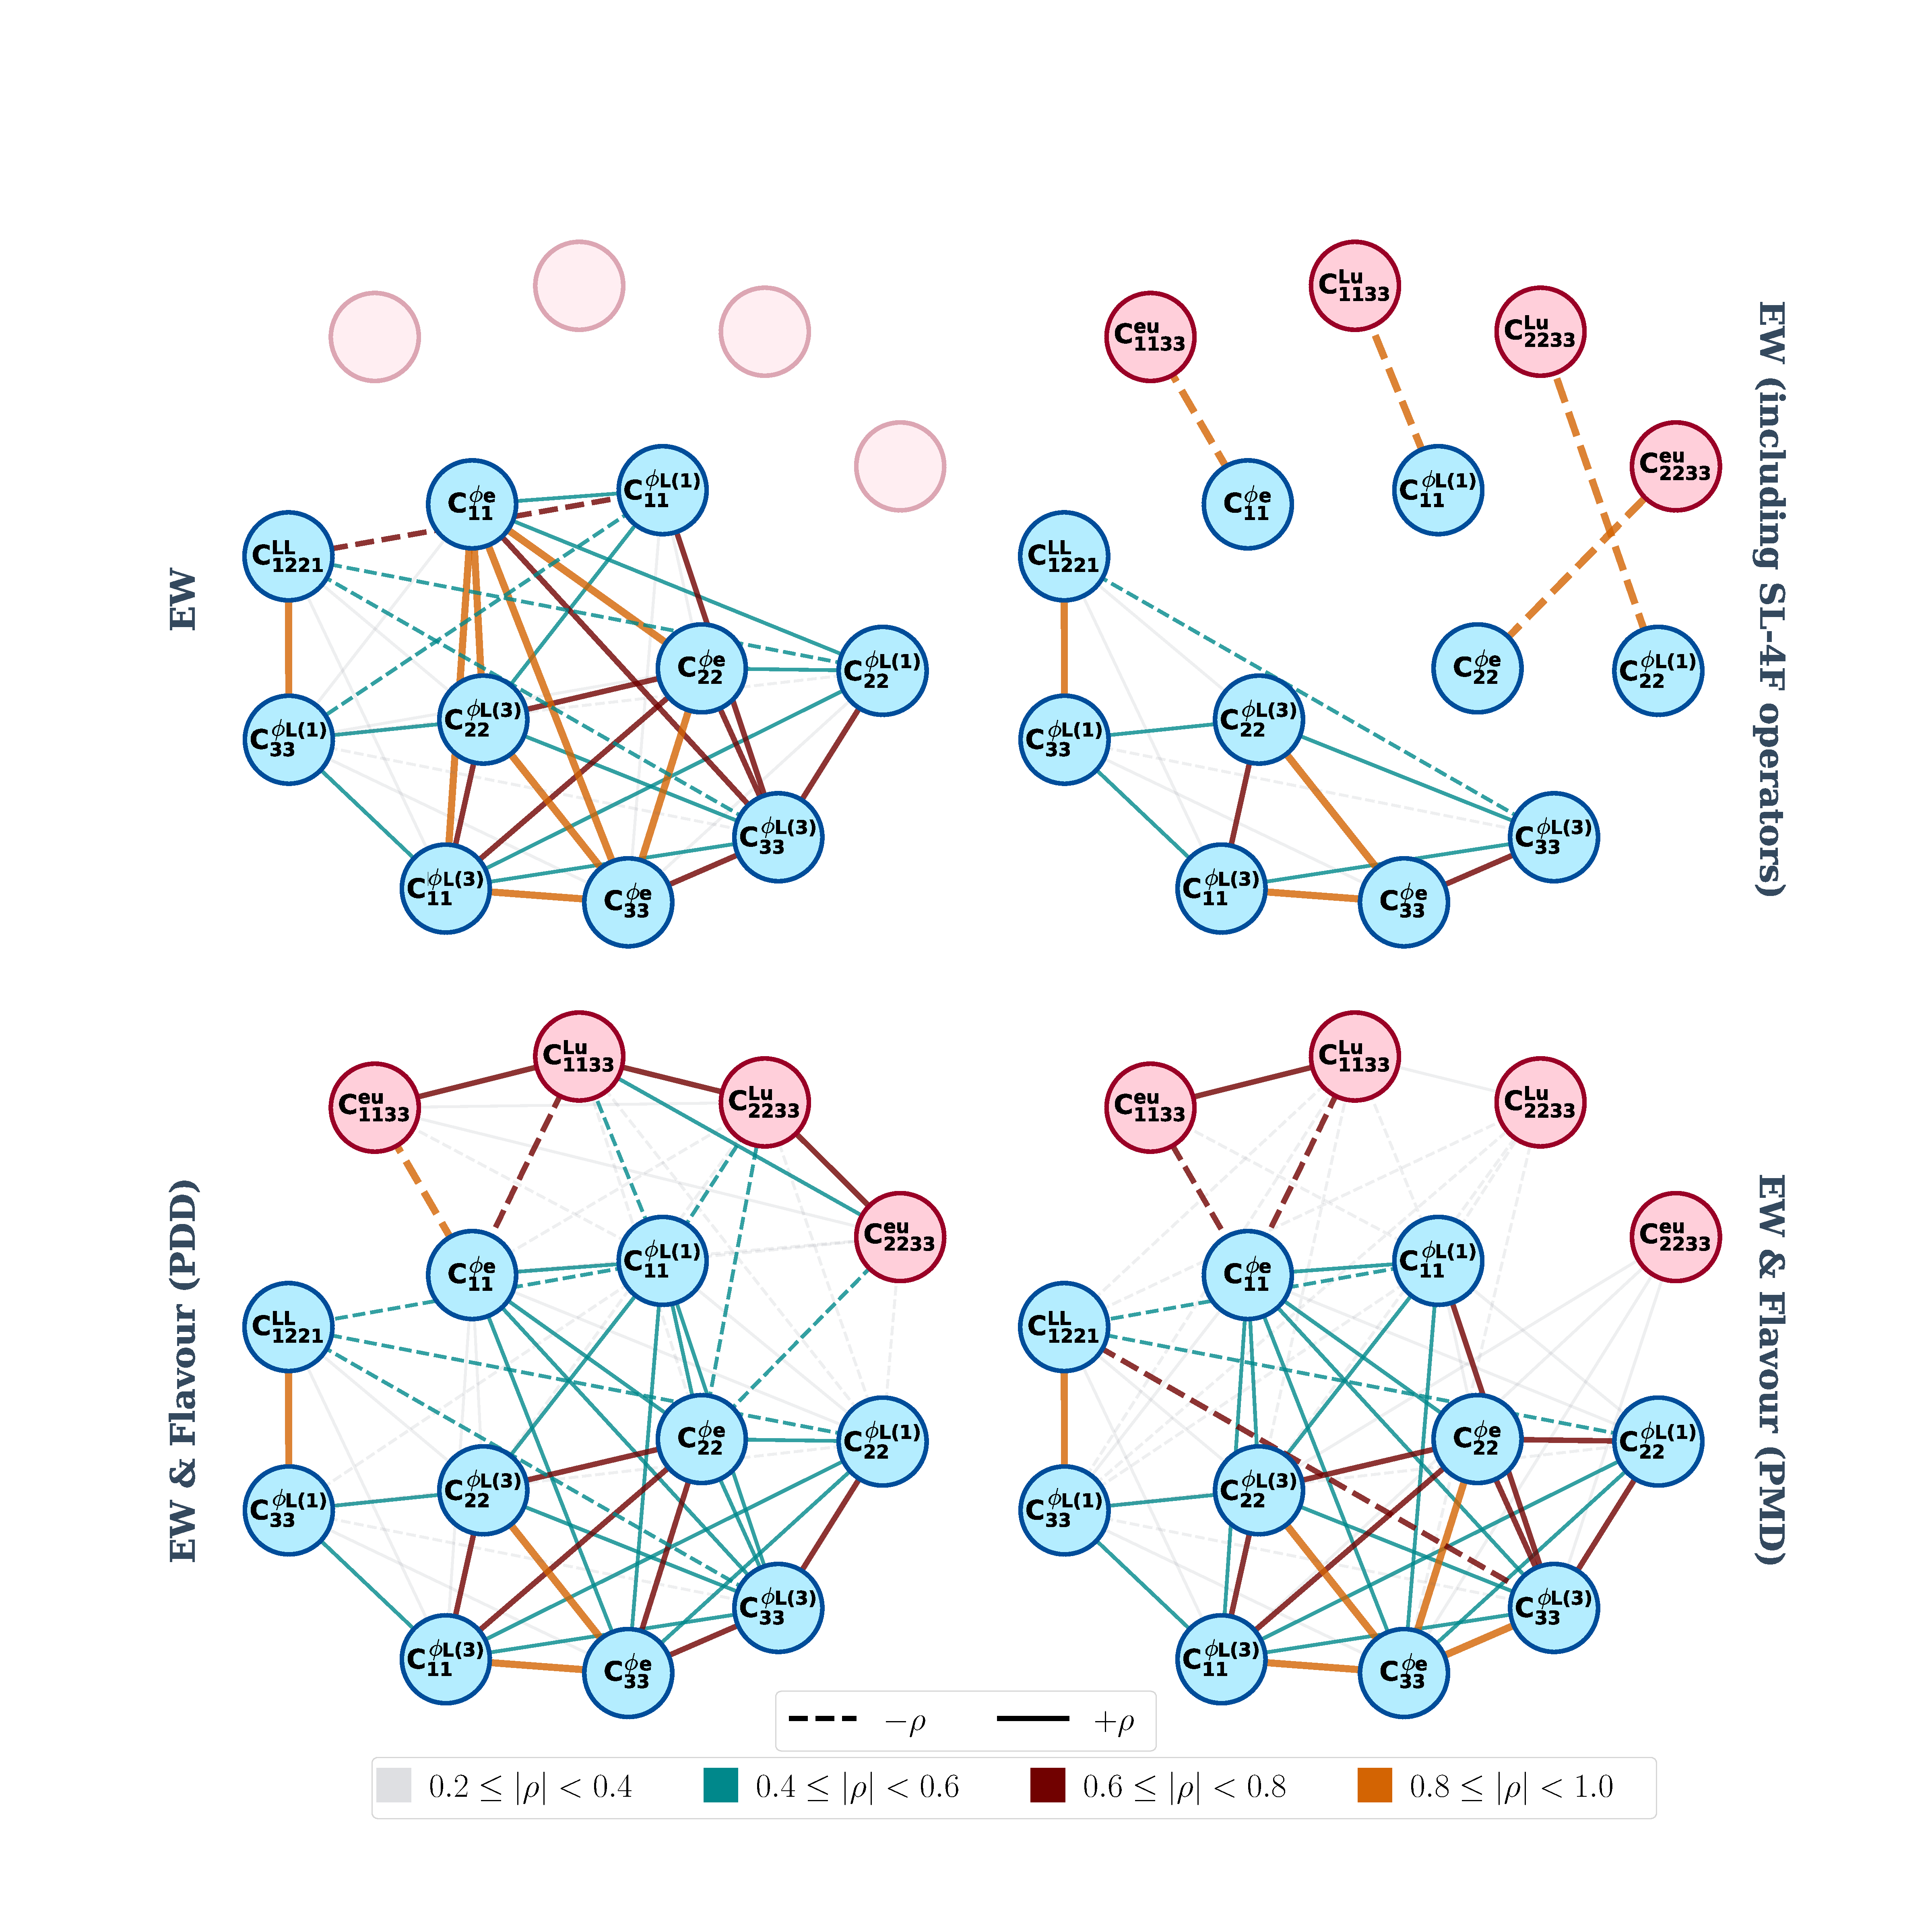
\includegraphics[width=0.9\textwidth]{figures/fixed_EW_flavour.pdf}
	\caption{ Network plot of the correlation between the Wilson coefficients considered in this study. The upper left panel shows the correlations from the \textbf{EW} fit, the upper right panel for the same fit but with the SL-4F Wilson coefficients included in the fit. The lower panel includes the flavour anomalies data in the \textbf{EW+Flavour}  scenario, in which the degeneracy is broken. The lower left panel is for the PDD hadronic effects, while the lower right one is for the PMD case. This figure is published in~\cite{Alasfar:2020mne}. 
	}
	\label{fig:ew_flav_corr}
\end{figure}
%\subsection{A minimal EFT picture}
It is not necessary to invoke all of the 21 SMEFT operators considered in the { EW \& Flavour} scenario to have a resolution for the flavour anomalies and EWPO. A simpler picture using two or four operators satisfies the experimental need to explain LUV and respect EW measurements. This picture contain the fully left-handed operator, $\mathcal{O}_{LQ}^{\ell \ell 2 3}$ and $\mathcal{O}_{\phi L}^{(1)} \ ^{\ell \ell}$. The former operator would be generated at a loop-level by $\mathcal{O}_{Lu}^{\ell \ell 3 3}$, while the latter at the tree level.  This minimalist SMEFT approach would then include only  $\mathcal{O}_{\phi L}^{(1)} \ ^{\ell \ell}$ and $\mathcal{O}_{Lu}^{\ell \ell 3 3}$, and $\ell= \mu, e$. So the model could involve either muons, electrons or both of them.\\ 
In~ \autoref{fig:2D_correlations}, the EWPO (grey), flavour with PDD (orange) and combined (magenta) fits for this minimal SMEFT model. For the muonic (left) and electronic (right) solutions. We observe the tension between EWPO and $b \to s \ell \ell$ data if individual fits were performed, which is resolved in the combined fit. However, this induces a correlation between the four-fermion operator $\mathcal{O}_{Lu}^{\ell \ell 3 3}$ and the one involving the Higgs-doublet and lepton bilinears. This model also obeys MFV assumptions, protecting it from other flavour observables. However, as mentioned earlier, the $B$ anomalies have to be explained at the one-loop level. 
\begin{figure}[htpb!]
	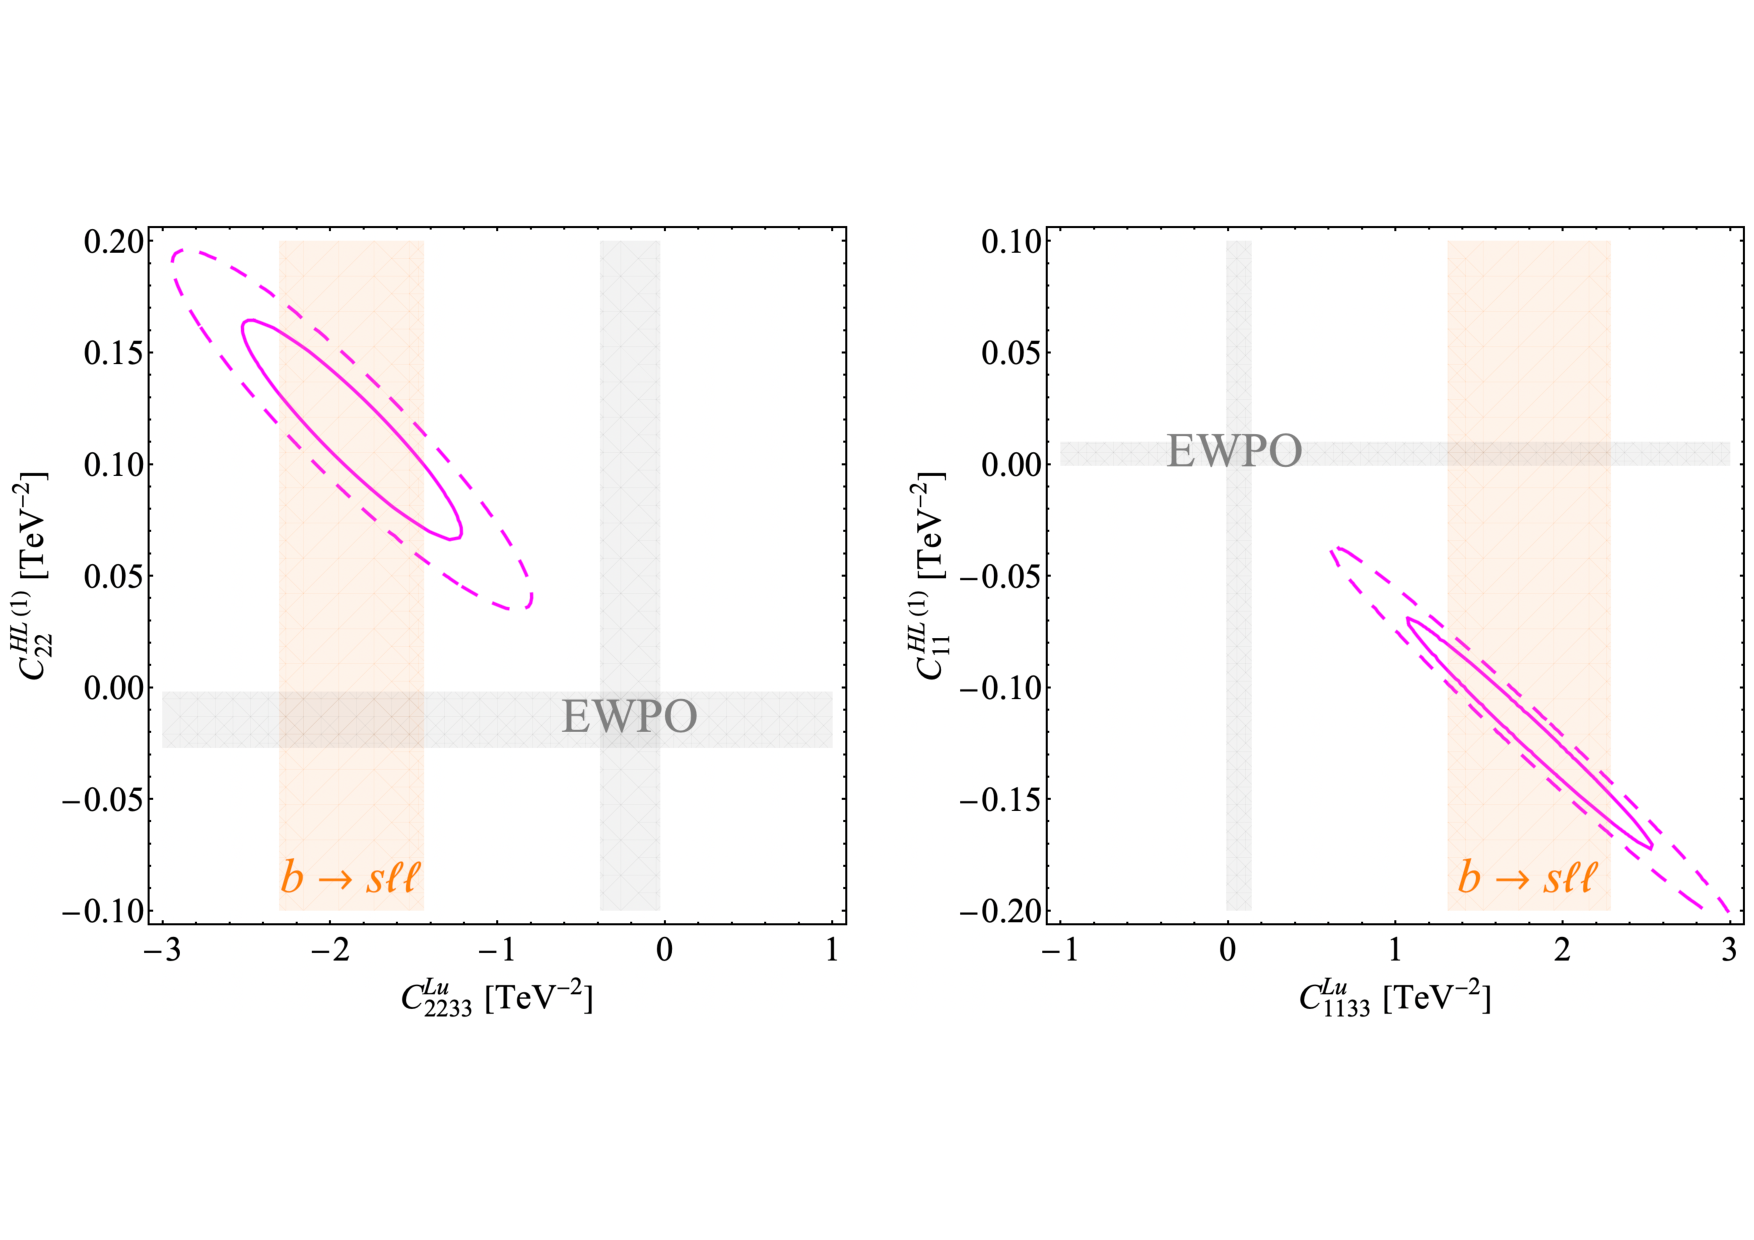
\includegraphics[width=\textwidth]{figures/CHL_CLu.pdf}
	\caption{ A minimal solution for the flavour anomalies within SMEFT while respecting EWPO. The left panel shows the four-fermion operators involving the muon, and on the right, the electronic solution is shown. EWPO fits are the grey regions, while the $b \to s\ell \ell$ measurements fits with PDD ansatz are highlighted by the orange bands. The combined fit's 1 and 2$\sigma$ contours are magenta coloured. This plot has been published in~\cite{Alasfar:2020mne}.  } 
	\label{fig:2D_correlations}
\end{figure}
Finally, note that the role played here by $\mathcal{O}_{Lu}^{\ell \ell 3 3}$ could be shared, in part, with $\mathcal{O}_{eu}^{\ell \ell 3 3}$, depending on how much departure is required from the fully left-handed solution to $B$ anomalies. As already noted, this fact critically depends on the information stemming from the angular analysis of $B \to K^{*} \mu \mu$~\cite{Ciuchini:2019usw}. On general grounds, to relieve the bounds from EWPO, the presence of $\mathcal{O}_{eu}^{\ell \ell 3 3}$ would also necessitate sizeable NP effects from $\mathcal{O}_{\phi e}^{\ell \ell}$, thus leaving us with a maximum of four needed operators to explain the flavour anomalies without being excluded by EWPO or including complex flavour structures.
%%%%%%%%%%%%%%%%%%
\section{\texorpdfstring{Z$^{\prime}$}{Z'} with vector-like partners}
\label{sec:mod_Zprime}
%In this section, we discuss how the lesson derived from the SMEFT picture illustrated, particularly in \autoref{fig:2D_correlations}, can be realised in a minimal extension of the SM. Here, we explicitly show how models involving a new $Z^\prime$ gauge boson around the TeV scale provide the most economical example of the correlations advertised in the previous section. 
%This can be achieved if we have a $Z^\prime$ coupled both to top and lepton SM fields.
%These couplings can be obtained by introducing vector-like top and muon/electron partners reasonably close to the EW scale~\cite{Kamenik:2017tnu,Fox:2018ldq}, making this class of models potentially interesting also from the point of view of naturalness in the Higgs sector.
%Finally, we will also briefly comment on possible alternative scenarios obtained with leptoquarks.
%%%%%%%%%%%%%%%%%%
Exhilarated by the SMEFT fit and the consequent simplified model discussed in the previous section, we discuss some UV-complete models that explain the $B$-anomalies at the loop level; without adding extra flavour violation; and respect the EWPO bounds.  \\  The first model that satisfies these requirements is based on a $Z^\prime$ model published in ref.~\cite{Kamenik:2017tnu}.  This model is a simple extension of the SM gauge group by an additional Abelian group $U(1)_X$ with a corresponding gauge boson $\mathsf{X}_{\mu}$ identified as the $Z^\prime$. All of the SM fields have no $X$ charge. This gauge symmetry is spontaneously broken by a vev of an additional scalar singlet $\mathsf{S}$, which gives a mass to the $Z^\prime$ boson~$m_{Z^{\prime}} = g_{X} \langle \mathsf{S} \rangle $. A top-quark~$\mathsf{T}$, (VLQ) and a muonic partners~$\mathsf{M}$ are added as well. These two fields mix with the top~$u_3$ and muon~$L_2$ via Yukawa interaction terms with the scalar field $\mathsf S$. Kinematic mixing between the $Z^\prime$ and the SM $Z$ boson and between the Higgs and the new scalar are assumed to be negligible. The new fields and their representation under the SM plus the new gauge group are summarised in~\autoref{tab:zrpime}. \\
This model is completely characterized by eight new parameters: the gauge coupling $g_{X}$, the mass $\mu_{\mathsf{S}}$ and quartic $\lambda_{\mathsf{S}}$ of the renormalizable potential of $\mathsf{S}$, the new Yukawa couplings $Y_{\mathsf{T},\mathsf{M}}$, here taken to be real, and the vector-like mass-term parameters $M_{\mathsf{T},\mathsf{M}}$.
In particular, the Lagrangian of the model contains the following terms:
\begin{align}
	\label{eq:new_Yukawa_Mu}
	\mathcal{L} &=
	M_{\mathsf{T}} \bar{\mathsf{T}}_R \mathsf{T}_L + M_{\mathsf{M}} \bar{\mathsf{M}}_R \mathsf{M}_L +
	Y_{t} \bar{u}_{3} \tilde{\phi}^\dagger Q_{3}  \nn \\ \qquad&+ Y_{\mathsf{T}} \bar{u}_{3} \mathsf{T}_L \mathcal{S} 
	+ Y_{\mu} \bar{e}_{2}  \phi^\dagger  L_{2}
	+ Y_{\mathsf{M}}\bar{\mathsf{M}}_R L_{2} \mathsf{S} + \mathrm{h.c.}  \ .
\end{align}
\begin{table}[htpb!]
	\centering
	\begin{tabular}{cc}
		\toprule
		Particle/Field& $G_\SM \otimes U(1)_X$ multiplicity  \\
		\midrule
		\topmidheader{2}{\textbf{VL fermions}} 
		$\mathsf{T}$ & $(\irrep{3},\irrep{2})_{Y={1\over 6},X={-1} }$\\
		$\mathsf{M}$ & $(\irrep{1},\irrep{2})_{{1\over 2},{-1} }$\\
		\midrule
		\topmidheader{2}{\textbf{Gauge boson}} 
		$\mathsf{X}_\mu$ & $(\irrep{1},\irrep{1})_{{0},{0} }$\\
		\midrule
		\topmidheader{2}{\textbf{Scalar}} 
		$\mathsf{S}$ & $(\irrep{1},\irrep{1})_{{0},{1} }$\\
		\bottomrule
	\end{tabular}   
	\caption{The added fields of this model and their representation under the SM gauge group and the new $U(1)_X$.Note that the  new charge assignment here is not unique, and the model would produce the same phenomenology with different but consistent assignment. }\label{tab:zrpime}
\end{table}
From this Lagrangian, we can read off the mixing terms between the SM fields and vector-like~(VL) partners.\footnote{Note that upon an opposite $U(1)_{X}$ charge assignment for the vector-like fermionic partners than the one implicitly assumed, one should replace in eq.~\eqref{eq:new_Yukawa_Mu} $\mathsf{S}$ with $\mathsf{S}^{\dagger}$.}
The spontaneous symmetry breaking of $U(1)_X$ is achieved in the way discussed at the beginning of this thesis in~\autoref{sec:ssb} by a non-vanishing vev $\langle \mathsf{S} \rangle^2 = -\mu^2_{\mathsf{S}}/(2 \lambda_{\mathsf{S}}) \equiv \eta^2 \neq 0$, that implies the following fermionic mixing patterns:
\begin{eqnarray}
	\label{eq:Mixing_Partner}
	& \textrm{top sector:} & \ 
	\left(  \begin{array}{cc}
		\bar{u}_3 & \overline{\mathsf{T}}_R
	\end{array} \right) \, \begin{pmatrix}
		\frac{Y_t  \, v}{\sqrt{2}} \ &  \frac{Y_{\mathsf{T}} \eta}{\sqrt{2}} \ \\
		0 \ & \ M_\mathsf{T}
	\end{pmatrix} \,
	\left(  \begin{array}{c}
		U_3 \\  \mathsf{T}_L
	\end{array} \right) \ + \ \mathrm{h.c.} \, , \\
	& \textrm{muon sector:} & \ 
	\left(  \begin{array}{cc}
		\bar{e}_2 & \overline{\mathsf{M}}_{R}
	\end{array} \right) \, \begin{pmatrix}
		\frac{Y_\mu v}{\sqrt{2}} \ & 0\ \\
		\frac{Y_{\mathsf{M}} \eta }{ \sqrt{2}}  \ & \ M_\mathsf{M}
	\end{pmatrix} \,
	\left(  \begin{array}{c}
		E_{2} \\  \mathsf{M}_L
	\end{array} \right) \ + \ \mathrm{h.c.} \, , \nonumber
\end{eqnarray}
where $U_{i}$ ($E_{i}$) indicates the $Q_{i}$-component ($L_{i}$-component) with weak isospin $1/2$ (-1/2). Using the determinant and trace of the squared mass matrices, one can easily show that the eigenvalues $m_{t,\mathsf{T}}$ and $m_{\mu,\mathsf{M}}$ must satisfy~\cite{Kamenik:2017tnu}:
\begin{eqnarray}
	\label{eq:Mass_Eigenvalues}
	m_{t,\mu} \,  m_{\mathsf{T,M}} & = & \frac{1}{\sqrt{2}} Y_{t,\mu} v M_{\mathsf{T,M}} \ , \\ m_{t,\mu}^2 + m_{\mathsf{T,M}}^2 & = & 
	M_{\mathsf{T,M}}^2 + \frac{1}{2} (Y_{t,\mu} \, v)^2 + \frac{1}{2} (Y_{\mathsf{T,M}} \, \eta)^2 \ , \nonumber
\end{eqnarray}
that in the decoupling limit clearly yield: $m_{t,\mu} \simeq Y_{t,\mu} v / \sqrt{2}$, $m_{\mathsf{T,M}} \simeq M_{\mathsf{T,M}}$.
Defining for the top sector the rotation matrix from the interaction to the mass basis following the convention:
\begin{equation}
	\label{eq:rot_phys_states} 
	\left(  \begin{array}{c}
		t_{R (L)} \\  \mathsf{T}^{\prime}_{R (L)}
	\end{array} \right) = \,
	\begin{pmatrix}
		\cos \theta^{t}_{R(L)} \ & \ - \sin \theta^{t}_{R(L)} \ \\
		\sin \theta^{t}_{R(L)}  \ & \ \ \ \, \cos \theta^{t}_{R(L)}
	\end{pmatrix} \,
	\left(  \begin{array}{c}
		u_{3} (U_{3}) \\  
		\mathsf{T}_{R (L)}
	\end{array} \right) \ ,
\end{equation}
and doing similarly for the muonic sector, the mixing angles between SM fields, $t$ and $\mu$,  and their partner mass eigenstates, $\mathsf{T}^{\prime}$ and $\mathsf{M}^{\prime}$, can be conveniently expressed in terms of the dimensionless ratios $\xi_{\mathsf{T,M}}$ and $\varepsilon_{t,\mu}\, $:
\begin{eqnarray}
	\label{eq:partner_mixing}
	& \  \tan 2 \theta_{R}^{t} = \frac{2 \xi_{\mathsf{T}}}{\xi_{\mathsf{T}}^2-\varepsilon_{t}^2-1} \, , \, 
	\ \, \tan 2 \theta_{L}^{t} = \frac{2 \varepsilon_{t}}{\xi_{\mathsf{T}}^2-\varepsilon_{t}^2 +1} \, , \,   \textrm{with} \ \varepsilon_{t} \equiv \frac{Y_{t} v}{Y_{\mathsf{T}} \eta},~\xi_{\mathsf{T}} \equiv \frac{\sqrt{2} M_{\mathsf{T}}}{\eta Y_{\mathsf{T}}} \, ; \ \\
	& \  \tan 2 \theta_{R}^{\mu} = \frac{2 \varepsilon_{\mu}}{\xi_{\mathsf{M}}^2-\varepsilon_{\mu}^2+1} \, , \, 
	\tan 2 \theta_{L}^{\mu} = \frac{2 \xi_{\mathsf{M}}}
	{\xi_{\mathsf{M}}^2-\varepsilon_{\mu}^2 -1}  \, , \, 
	\textrm{with} \ \varepsilon_{\mu} \equiv \frac{Y_{\mu} v}{Y_{\mathsf{M}} \eta},~\xi_{\mathsf{M}} \equiv \frac{\sqrt{2} M_{\mathsf{M}}}{\eta Y_{\mathcal{M}}} \, .
	\nonumber
\end{eqnarray}
In a perturbative expansion in $\varepsilon_{t,\mu}$, eq.~\eqref{eq:partner_mixing} clearly shows that the mixing in the top sector proceeds mainly through $\tan\theta^{t}_{R} \simeq 1/\xi_{\mathsf{T}}$, while in the muonic sector one has  $\tan\theta^{\mu}_{L} \simeq 1/\xi_{\mathsf{M}}$ and negligible $\tan\theta^{\mu}_{R}$.

Hence, for $\varepsilon_{t,\mu}/\xi_{\mathsf{T,M}}= Y_{t,\mu} v/\sqrt{2} M_{\mathsf{T,M}} < 1$, the leading couplings of the $Z^{\prime}$ boson to the SM fields correspond to right-handed top-quarks and to left-handed muons as well as neutrinos, these couplings are given by
\begin{eqnarray}
	\label{eq:Zprime_to_SM}
	g_{Z^{\prime} t_{R}} & = & g_{X} \sin^2 \theta_{R}^{t} = \frac{g_{X}}{ 1+ \xi^2_{\mathsf{T}}} + \mathcal{O}\left( \varepsilon_{t}^2/\xi_{\mathsf{T}}^2 \right) \, , \\
	g_{Z^{\prime} \mu_{L} (\nu)} & = &  g_{X} \sin^2 \theta_{L}^{\mu} = \frac{g_{X}}{1 + \xi^2_{\mathsf{M}}} 
	+ \mathcal{O}\left( \varepsilon_{\mu}^2 /\xi_{\mathsf{M}}^2 \right) \, ,
\end{eqnarray}
with $g_{Z^{\prime} t_{L} (\mu_{R})}$ contributing only at order $\varepsilon_{t  (\mu)}^2/\xi_{\mathsf{T(M)}}^2$.
\begin{figure}[htpb!]
	\centering
	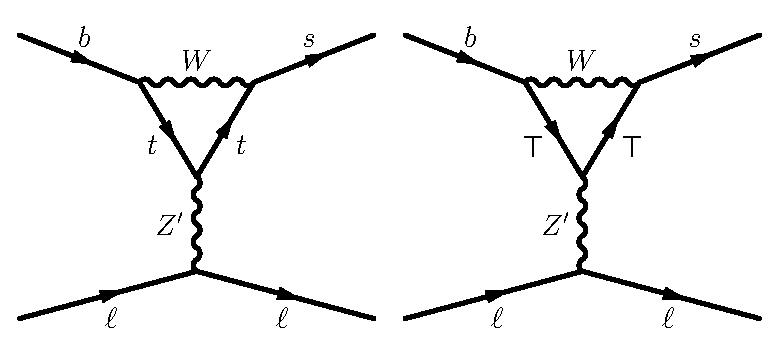
\includegraphics[scale=.75]{figures/zp_penguin.pdf}
	\caption{FCNC penguins with LUV emerging from the $Z^\prime$ model, explaining the $b \to s \ell \ell$ anomalies at loop-level. The penguin diagrams with the top-partners in the loop are the dominant ones. }
	\label{fig:peng}
\end{figure}
The $ b \to s \ell \ell$ anomalies can be explained in this model via penguin (also box) diagrams with LUV as shown in~\autoref{fig:peng}. Since the $Z^\prime$ couples to the muons and not the electrons, LUV is generated at loop-level. 
%%%
\subsection{SMEFT matching and constraints}
Integrating out the $Z^{\prime}$ will generate the operator $\mathcal O_{L u}^{2233}$ with the the matching condition:
\begin{equation}
	\label{eq:CLu_Zprime}
	C_{L u}^{2233} = - \frac{g_{Z^{\prime} t_{R} } g_{Z^{\prime} \mu_{L}} }{m_{Z^{\prime}}^2} \simeq - \frac{1}{(1+ \xi^2_{\mathsf{T}})(1+ \xi^2_{\mathsf{M}}) \, \eta^{2}} \ ,
\end{equation}
%
Together with four-fermion operators built of $t_{R}$ or $\mu_{L},\nu$  fields that can be potentially probed at collider and by experimental signatures like $\nu$-trident production. 
From eq.~\eqref{eq:CLu_Zprime} it is clear that in order to have $|C_{L u}^{2233}| \sim 2 $ TeV$^{-2}$ as required  by the fit in \autoref{fig:2D_correlations}, the SSB of the new gauge group needs to happen at a scale close to the EW, namely $\eta \lesssim$~TeV;\footnote{Note that even for masses as low as $\mu_{\mathsf{S}} \sim \mathcal{O}(v)$, for $\eta \simeq v$ and $\lambda_{\mathsf{S}} \sim \mathcal{O}(1)$, the interactions of $\mathsf{S}$ do not alter the phenomenology discussed here since the largest $\mathcal{S}$-generated effects are still suppressed as $\mathcal{O}(\varepsilon_{t}^2/\xi^2_{\mathsf{T}})$.} for $m_{Z^{\prime}} \sim$~TeV this leads to a natural coupling~$g_{X} \gtrsim$~1. \\ The main collider constraints come from the production of top pair $ pp \to Z^\prime \to t \bar t$, with the most stringent bounds at the time of conducting this work came from ATLAS~\cite{ATLAS:2019npw}. In addition to the resonant di-muon searches~\cite{ATLAS-CONF-2019-001}. In~\autoref{fig:Zp_constraints1} these searches are projected onto our model, with the choice of $\eta=1$ TeV and other parameters chosen to be preferred by the $B$ anomalies observables, we see that the constraints on this model are dominated by the resonant di-muon searches. The theoretical prediction of the resonant top pair and di-muon production via gluon fusion $ gg \to Z^\prime \to t \bar t /\mu \mu$ in this model has been calculated at NLO using the two-loop triangle calculations presented in~\autoref{chap:hz}. Further emphasising the importance of calculating Higher-order corrections for the gluon fusion $ gg \to Z^*$ for NP processes on top of Higgs measurements. \\
In \autoref{fig:Zp_constraints} collects the constraints on this model, starting with the $1\sigma$ region corresponding to the explanation of $B$ anomalies via eq.~\eqref{eq:CLu_Zprime} in the parameter space $\xi_{\mathsf{T,M}}$, fixing the gauge coupling $g_{X} = m_{Z^{\prime}}/\eta$ for a tentative $Z^{\prime}$ gauge boson at the~TeV scale and the VEV of the new scalar field $\mathsf{S}$ set to $\eta = 250$~GeV and $\eta = 500$~GeV  in the left and right panel, respectively. In the same plot, the collider searches are also presented, re-interpreted from the results presented in ref.~\cite{Camargo-Molina:2018cwu}. 
\begin{figure}[htpb!]
	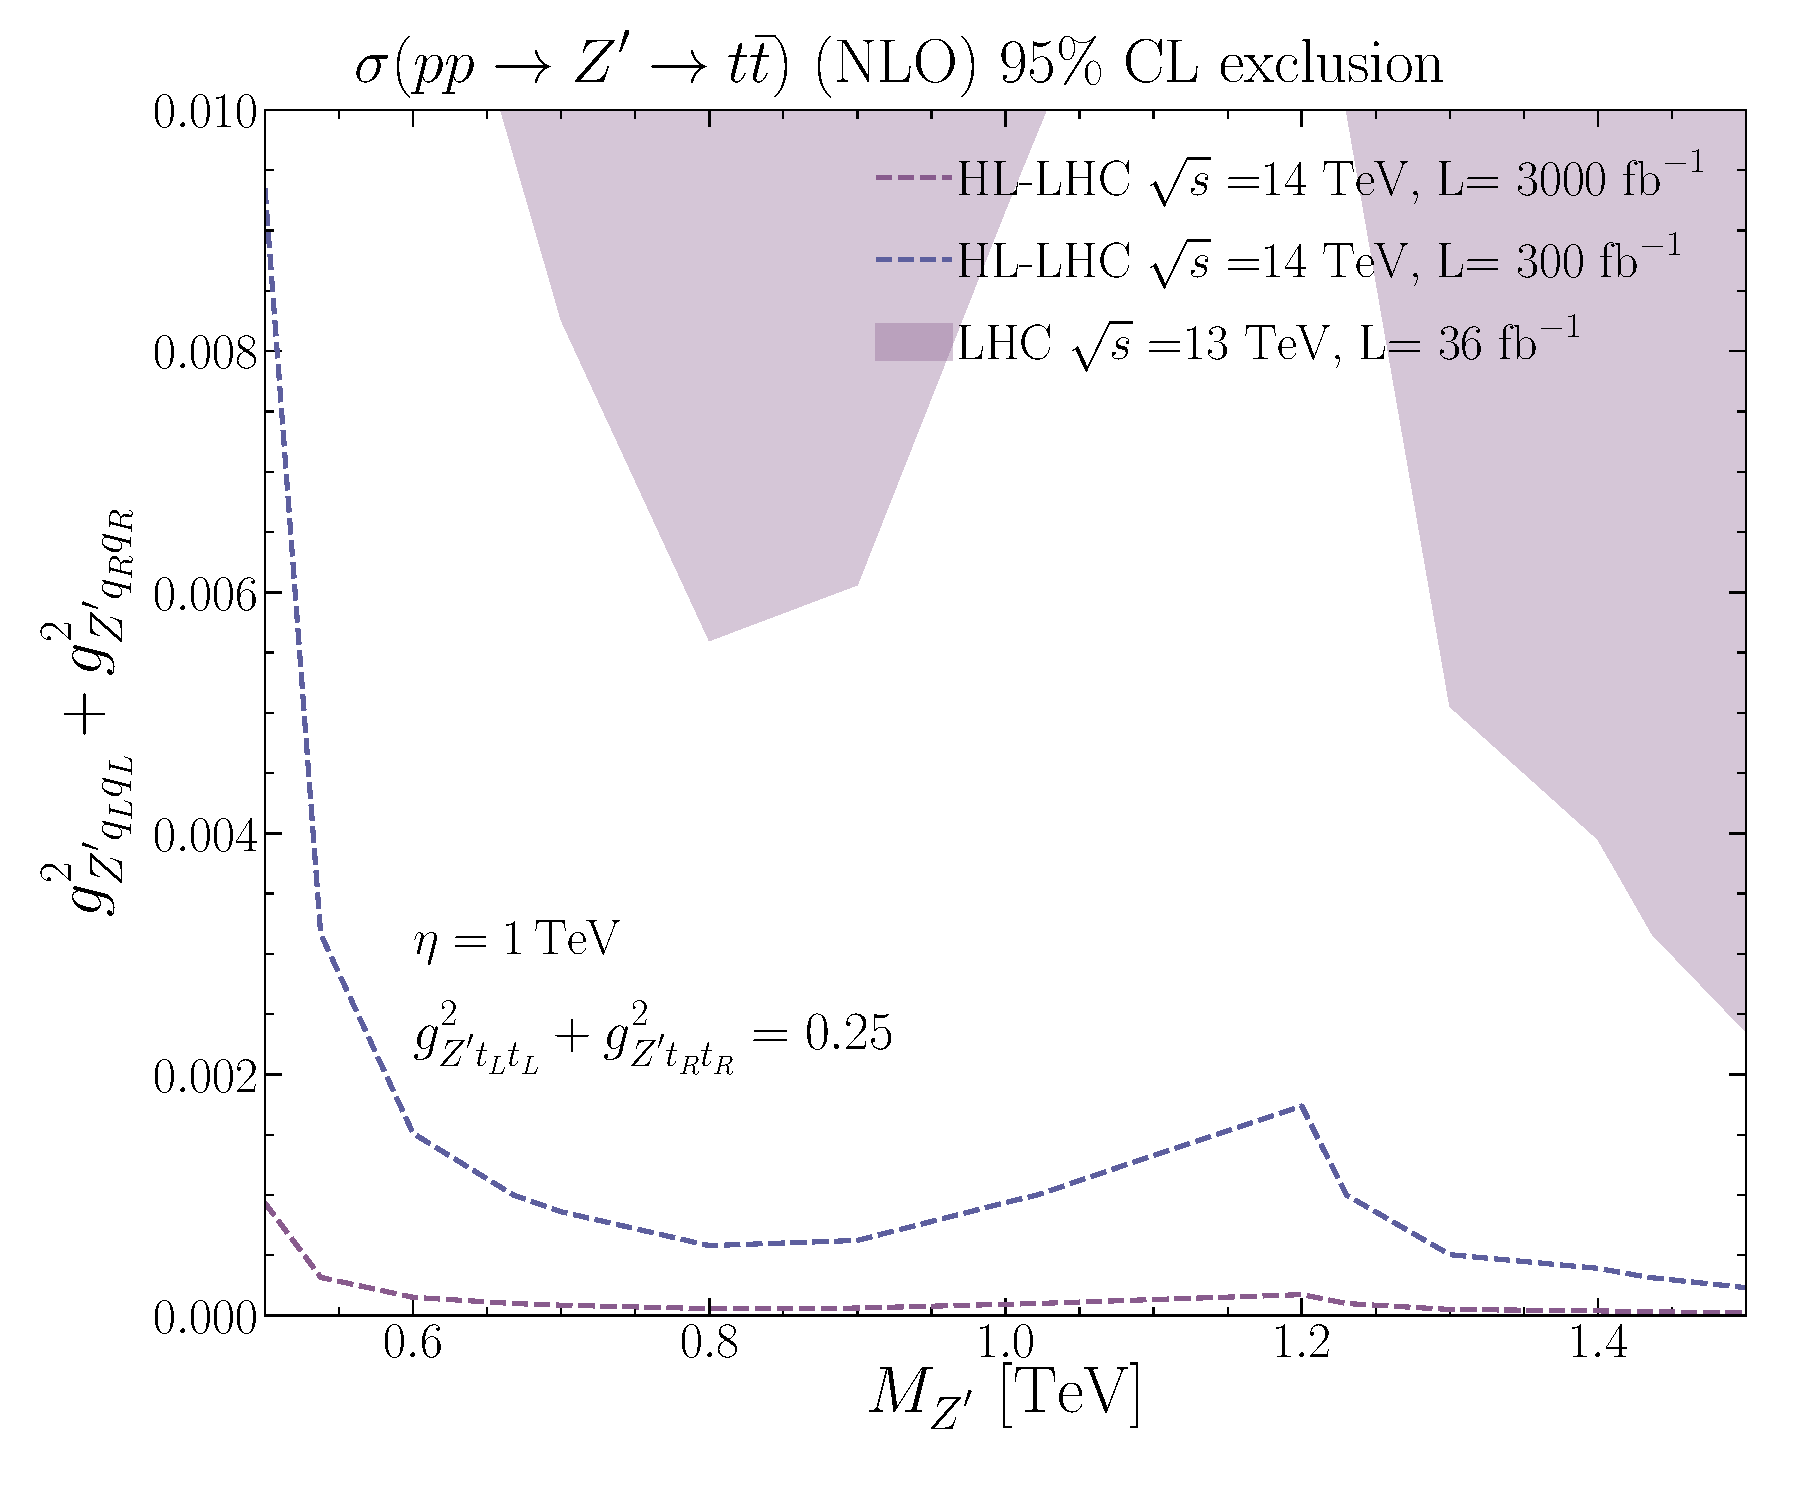
\includegraphics[scale=0.235]{figures/bounds_xs.pdf}
	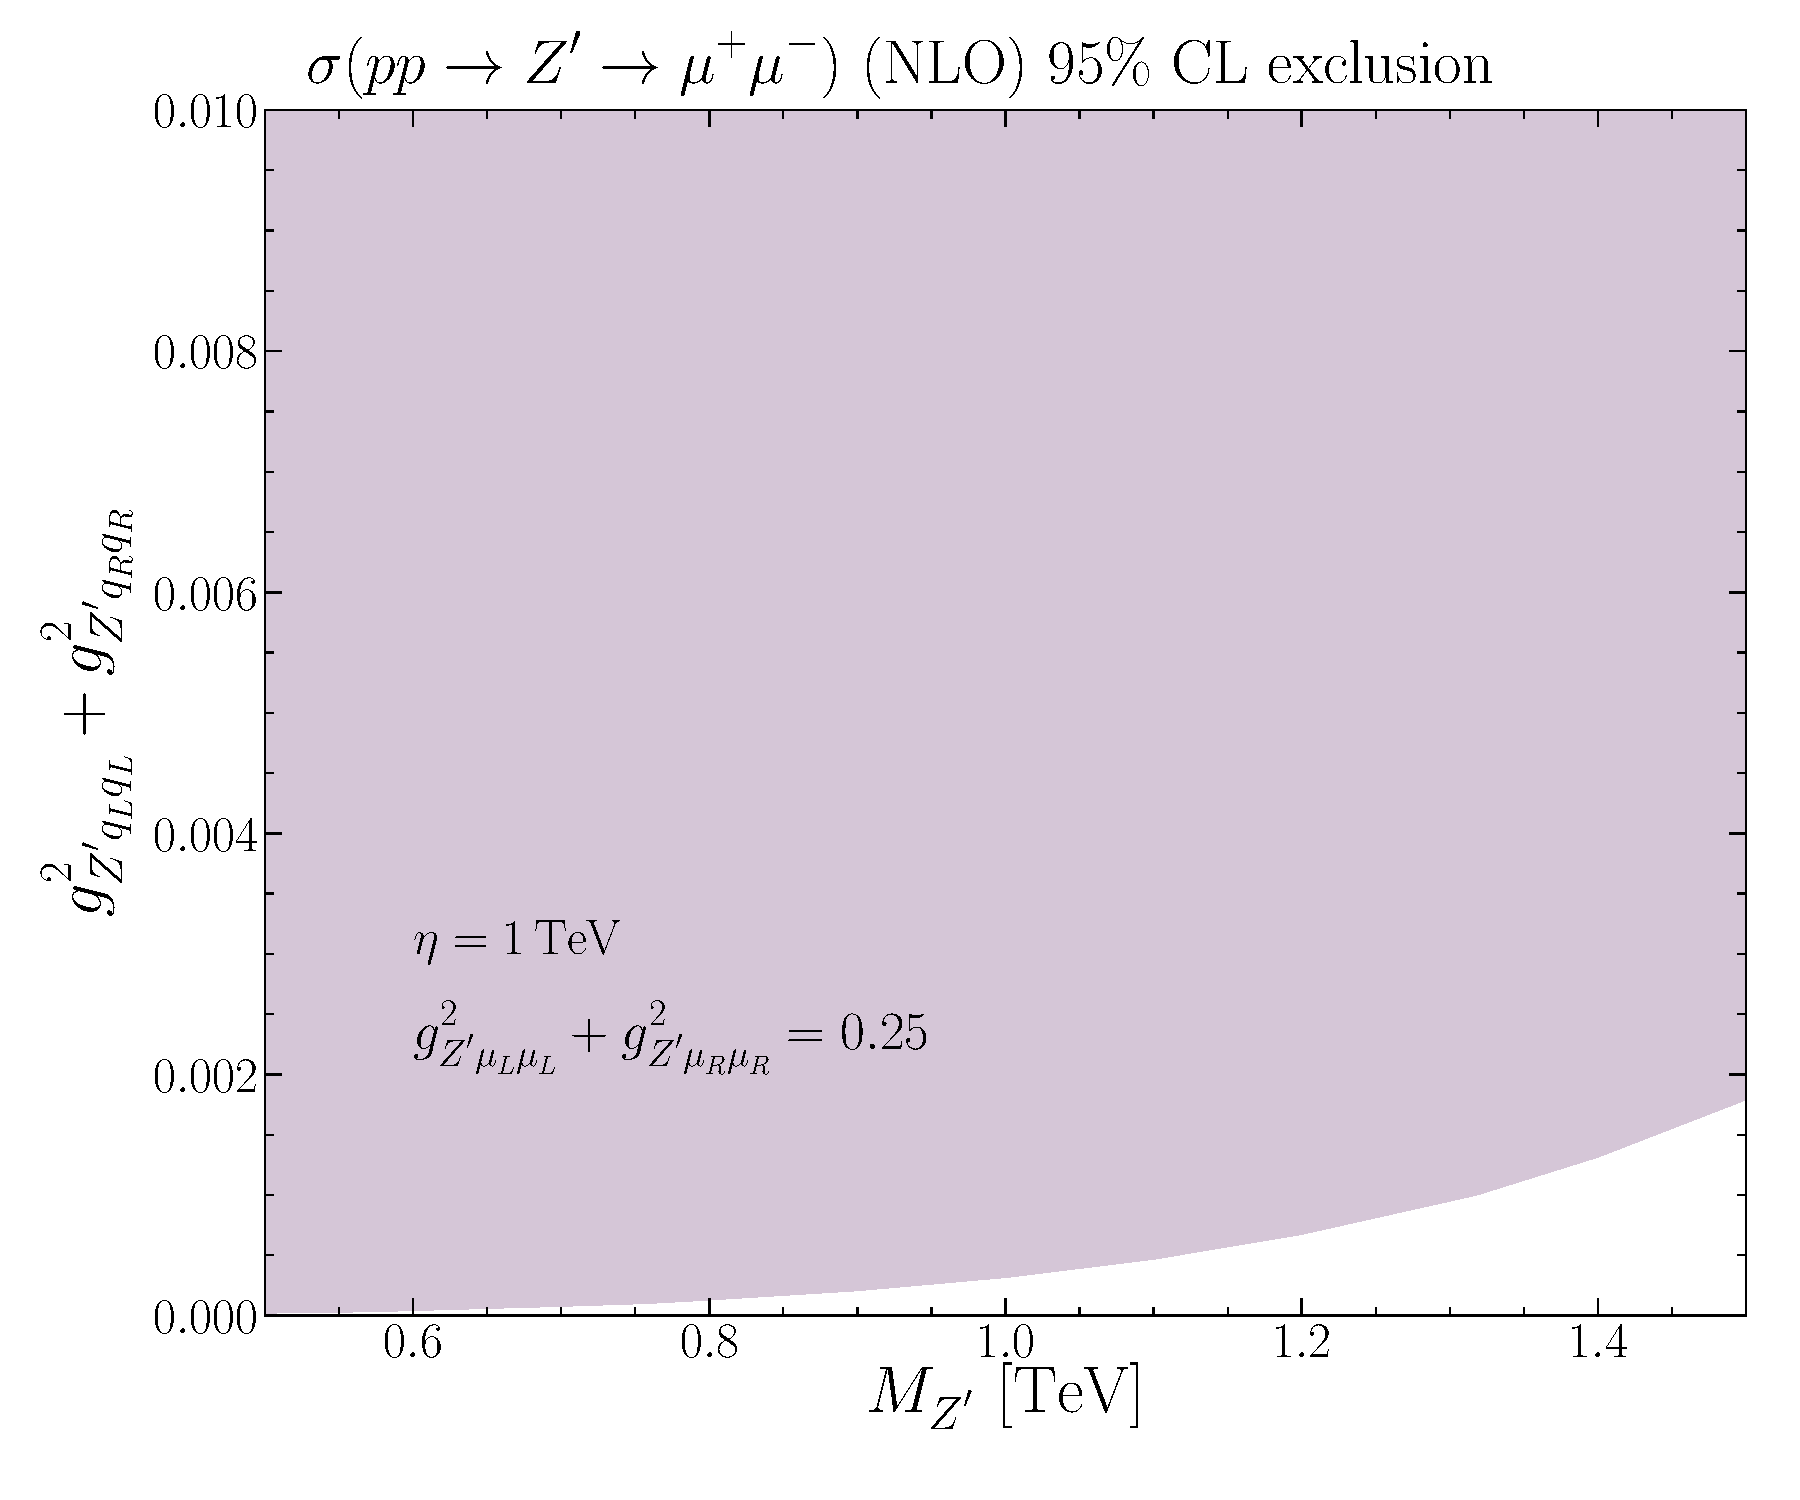
\includegraphics[scale=0.235]{figures/zmumu.pdf}
	\caption{Direct searches for $Z^\prime$ using top pair production~\cite{ATLAS:2019npw} and di-muon searches~\cite{ATLAS:2019npw}, the gluon fusion cross-sections for this model were calculated at NLO using the results of the two-loop triangle calculations of the process $ gg \to Z^*$ preformed in~\autoref{chap:hz}.}
	\label{fig:Zp_constraints1}
\end{figure}
\begin{figure}[htpb!]
	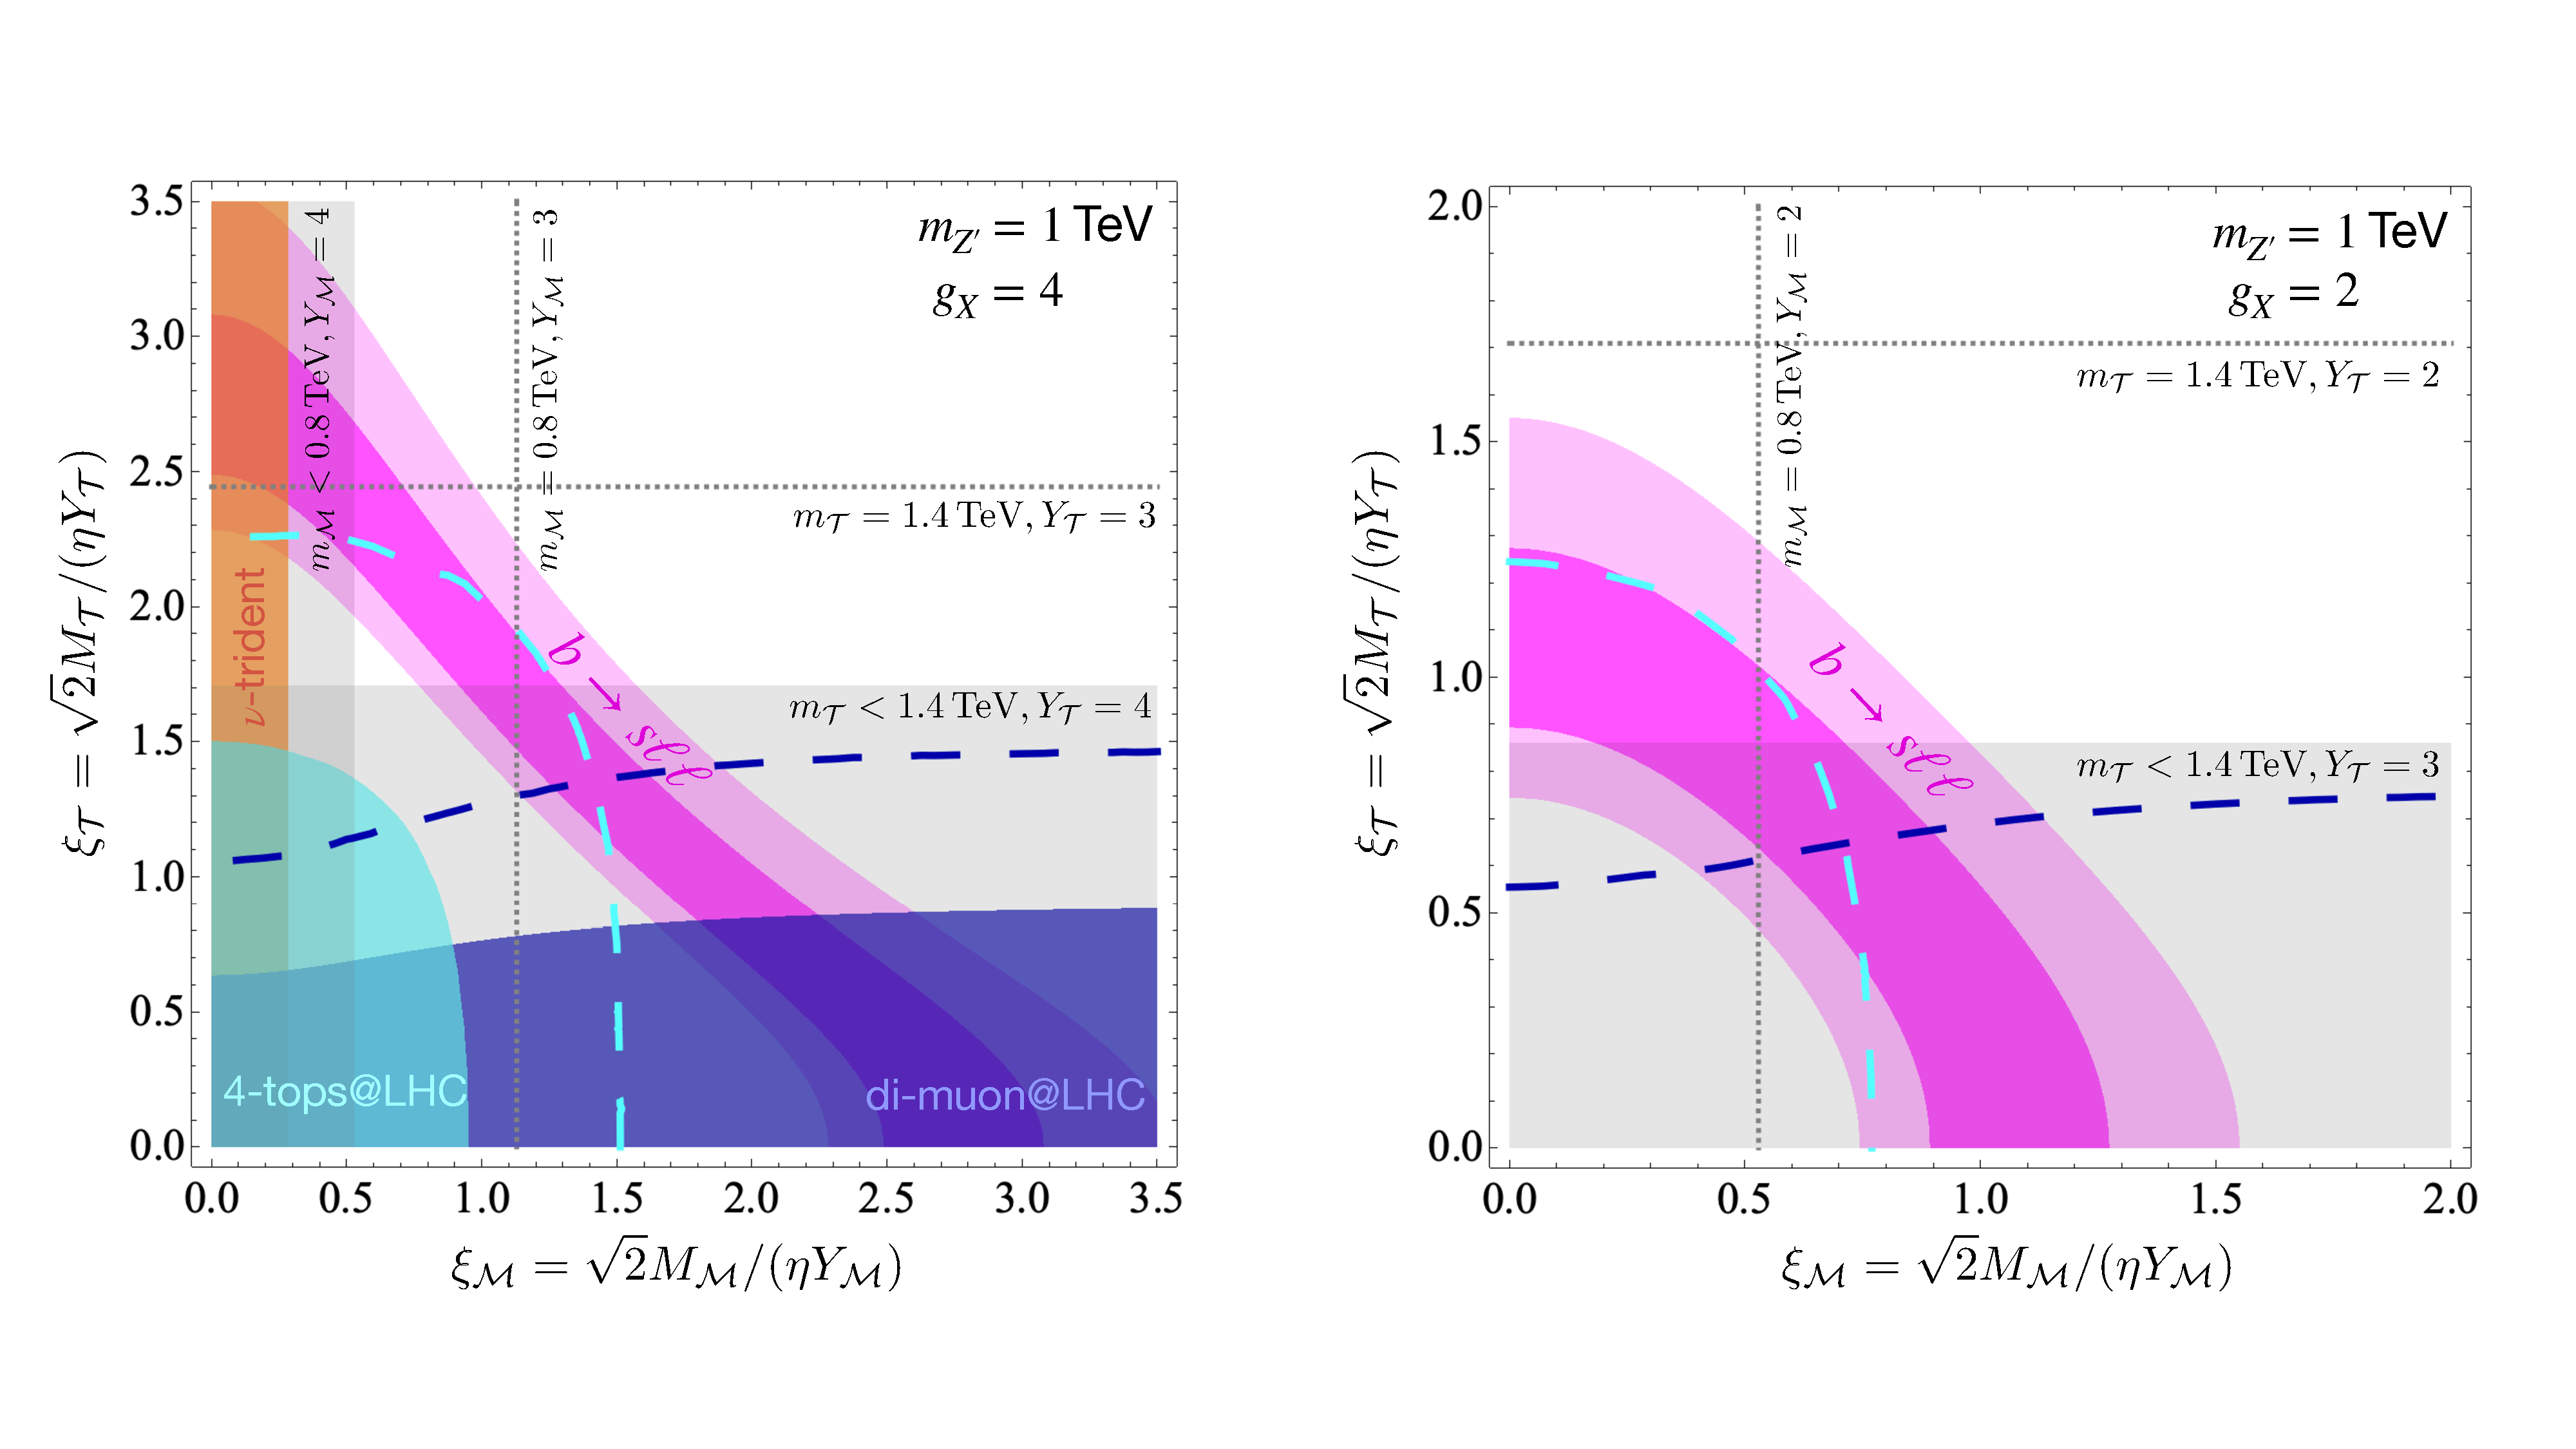
\includegraphics[scale=0.235]{figures/Zprime_constraint_CLu.pdf}
	\caption{ Collective of the constraints on the $Z^\prime$ model. the magenta regions show the  $68\%$ and $ 95\%$ CL  constraints from $ b \to s \ell \ell$ anomalies, while the rest are the collider searches re-interpreted from the ones in ref.~\cite{Camargo-Molina:2018cwu}. The projections for the early HL-LHC  (at 300~fb$^{-1}$) constraints are shown as dashed lines. Grey regions underlie the parameter space where the mass of the vector-like partner lies below current collider limits for a fixed Yukawa coupling as explicitly reported. At the same time, dashed lines show the corresponding shift of the limit due to a smaller value of the same type of Yukawa coupling. The left panel is for $\eta = m_Z^\prime /4$
		and the right panel is for $\eta = m_Z^\prime /2$. This figure is published in~\cite{Alasfar:2020mne}.}
	\label{fig:Zp_constraints}
\end{figure}
The bounds from neutrino-trident production performed in~\cite{Mishra:1991bv} constrain small $\xi_{\mathsf{M}}$, where the 95 \%CL bounds are shown in the orange band of the plot.  The top-phillic $Z^{\prime}$  is predominantly produced at tree-level in association with top-pair, in the blue region we show the 95\% high-$p_{T}$ constraint stemming from the recasting of the $p p \to \mu^{-} \mu^{+} t \bar{t}  $ search at ATLAS~\cite{Aaboud:2017buh,ATLAS-CONF-2019-001}. The cyan contours are constraints coming from four-tops production analysis from CMS~\cite{Sirunyan:2017roi}, see ref.~\cite{Camargo-Molina:2018cwu} for more details.  These constraints' prospects for the early runs of the HL-LHC at 300~fb$^{-1}$ are also explored and indicated with the dashed lines. One can see that the model benchmark is shown in the right panel of ~\autoref{fig:Zp_constraints} old promising potential for discovery at the HL-LHC. 
Finally, in the same figure, fixing the partner Yukawa coupling to  $\mathcal{O}(1)$ values as reported in the two panels, we mark in grey the region corresponding to the bound on the mass of the vector-like partner expected from collider, taken to be $m_{\mathsf{T}} = 1.4$~TeV from the search at ATLAS in ref.~\cite{Aaboud:2018uek}, and $m_{\mathsf{M}} = 0.8$~TeV from the CMS analysis of ref.~\cite{Sirunyan:2019ofn}.\\
%%%%%
\subsection{Expanding the model}
For this model to survive EWPO constraints, it needs to induce  $O_{\phi L}^{(1)}\ ^{22}$ with the same correlation patterns observed in\autoref{fig:2D_correlations}.  In principle, it is possible to achieve that by inducing tree-level $z-Z^\prime$ mixing by charging $\mathsf{S}$ under $U_Y(1)$ in addition to $U_X(1)$, thereby inducing some misalignment in the weak hypercharge $Y$. However, this will create a tree-level (Drell Yan-like) resonant di-muon production enhancement, far beyond what is allowed by current collider searches~\cite{ATLAS-CONF-2019-001}.  Therefore, this mechanism is not possible. \\ In order to accommodate for EW precision constraints, this model needs to be expanded further by including new VL leptonic states, like the ones discussed in refs.~\cite{Thomas:1998wy,delAguila:2008pw}. These new degrees of freedom are interesting by their own merit, in particular with resolving the anomaly associated with $(g-2)_{\mu}$~\cite{Kannike:2011ng,Muong-2:2021ojo}, also for neutrino mass source and other interesting collider phenomenology ~\cite{Kumar:2015tna,Bhattiprolu:2019vdu}.\\ 
The simplest resolution can be accomplished by the inclusion of  two new vector-like muonic partners: a singlet under $SU(2)_{L}$, $S_{Y}$, and a triplet of $SU(2)_{L}$, $T_{Y}$, 
where in both cases the subscript $Y$ denotes the hypercharge of the fermion. Since they are VL fermions, they have a mass term , thus adding new parameters~$M_{S_{Y},T_{Y}}$. Their mixing with the SM leptons comes -like $\mathsf{M}$- from Yukawa term, which for $Y=0$ is given by
\begin{equation}
	\label{eq:Yuk_singl_tripl}
	\mathcal{Y}_{S_{0}} \bar{S}_{0,R} \tilde{\phi}^{\dagger} L_{2} + \mathcal{Y}_{T_{0}} \bar{T}^{A}_{0,R} \tau^{A} \tilde{\phi}^{\dagger} L_{2} + \textrm{h.c.}  \ ,
\end{equation} 
Another possibility of interest may be the one of replacing in eq.~\eqref{eq:Yuk_singl_tripl} $\tilde{\phi} $
with the Higgs doublet, $\phi$, and then the pair of vector-like partners with hypercharge $Y=1$.  The matching condition for these new fields produces the needed SMEFT operators, and the values and sign of the corresponding Wilson coefficients are given by the interplay between these fields ~\cite{delAguila:2008pw,Kannike:2011ng} of the form:
\begin{eqnarray} 
	\label{eq:matching_CHL}
	C_{\phi L}^{(1)}\ ^{22 } & = &
	\ \ \frac{ \mathcal{Y}^{2}_{S_{0}}}{4 M_{S_{0}}^2} 
	- \frac{ \mathcal{Y}^{2}_{S_{1}}}{4 M_{S_{1}}^2}
	+ \frac{ 3 \mathcal{Y}^{2}_{T_{0}}}{4 M_{T_{0}}^2}
	- \frac{ 3 \mathcal{Y}^{2}_{T_{1}}}{4 M_{T_{1}}^2} \ , \\
	C_{\phi L}^{(3)} \ ^ {22} & = & 
	- \frac{ \mathcal{Y}^{2}_{S_{0}}}{4 M_{S_{0}}^2}
	- \frac{ \mathcal{Y}^{2}_{S_{1}}}{4 M_{S_{1}}^2}
	+ \frac{ \mathcal{Y}^{2}_{T_{0}}}{4 M_{T_{0}}^2}
	+ \frac{ \mathcal{Y}^{2}_{T_{1}}}{4 M_{T_{1}}^2} \ . \nonumber
\end{eqnarray}
In order to obtain the needed value and sign of  $C_{\phi L}^{(1)}\ ^{22} \sim 0.1$ but also vanishing or negligible  $C_{\phi L}^{(3)}\ ^{22}$ some tuning between the singlet and the $Y=0$ triplet is needed, although this tuning is stable under the RGE once generated at the NP scale. \\
Working under the PDD ansatz, it is possible to consider that the model would couple to the electron instead of the muon. Not much would change in terms of the particle content of this model, except for opposite charge assignment to get correct signs for the Wilson coefficients of $O^{Lu}$ and $O_{\phi L}^{(1)}$ seen in the right panel off~\autoref{fig:2D_correlations}, but making the electron and top partners having opposite $X$ charges and then making the proper adjustments to the Lagrangian. 
A final comment is needed for the electron scenario reported in the right panel of~\autoref{fig:2D_correlations}, that involves opposite signs for the Wilson coefficients of $O^{Lu}$ and $O_{\phi L}^{(1)}$ discussed so far. For the former, we note that the sign highlighted in the matching in eq.~\eqref{eq:CLu_Zprime} follows from having assumed the same sign for the charge of the vector-like top and muon partners under $U(1)_{X}$. For what concerns the generation of $C_{\phi L}^{(1)} \ ^{11} < 0 $, according to eq.~\eqref{eq:matching_CHL} one needs to correlate once again the contribution stemming from $S_{0}$, or from $S_{1}$, with the effect coming from a $SU(2)_{L}$ triplet, that now needs to be identified with $T_{1}$, namely the triplet of hypercharge $Y=1$.

%Eventually, we wish also to comment on the possible role of the $O_{eu}$ operator, so far neglected in this discussion, but of potential relevance more in general. As mentioned earlier, the presence of $O_{eu}$ would be particularly needed in the case where hadronic corrections entering in the amplitude of $B \to K^* \ell \ell $ would be of the size originally estimated in~\cite{Khodjamirian:2010vf}. 
%In that case, a solution to flavour anomalies would be preferred in the muonic channel with NP Wilson coefficient $C_{eu}^{2233}$ also substantially deviating from 0, as already discussed in \autoref{sec:GEN_EFT_results}. Then, one would need to involve also the operator $C_{\phi e}\ ^{22}$ to relieve possible tensions with EW precision. In a general picture, the required NP effects from $O_{\phi e}_{11,22}$ can be obtained by integrating out heavy vector-like $SU(2)_{L}$ leptonic doublets.

%%%%%%%%%%%%%%%%%%
\section{Leptoquark scenarios}
\label{sec:mod_Leptoquarks}
%%%%%%%%%%%%%%%%%%
Leptoquark models are generically predicted in grand unified  theories~(GUTs)~\cite{Pati:1974yy,PhysRevLett.32.438}. They typically generate a baryon violating process that leads to proton decay, which is severely constrained. However, in light of the simplified SMEFT model discussed earlier \autoref{fig:2D_correlations}, it is possible to introduce leptoquarks~(LQ) that couple non-universally to quark and lepton generations.  These LQs are within reach of colliders and not pushed to the GUT scale like their flavour-universal counterparts. Actually, they are potential candidates for explaining the flavour anomalies ~\cite{Camargo-Molina:2018cwu,Coy:2019rfr}.  Such models typically involve a highly non-trivial flavour structure.  For a comprehensive survey of LQ models, see for instance~\cite{Buchmuller:1986zs,delAguila:2010mx,Alonso:2015sja,Dorsner:2016wpm,deBlas:2017xtg}. \\
In this section, we limit ourselves to LQs that generate  $C_ {Lu}^{\ell \ell33}$ and $C_{eu}^{\ell \ell33} $, and introduce LUV in $b \to s \ell \ell$ transition at loop-level as shown in~\autoref{fig:lqflav}. With that in mind, only a handful of LQs models remain; they are summarised in ~\autoref{tab:LQmodels}.
\begin{figure}[htpb!]
	\centering 
	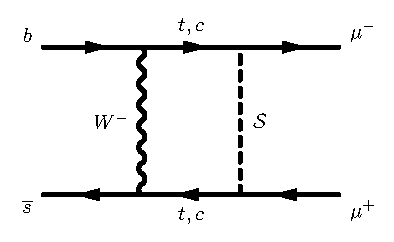
\includegraphics[width=0.45\linewidth]{figures/x_bsllSLQ}
	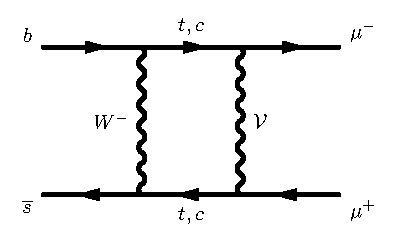
\includegraphics[width=0.45\linewidth]{figures/x_bsllVLQ}
	\caption{Box diagrams generates by scalar $\mathcal S$ (left) and vector $\mathcal V$ leptoquarks, of the $b \to s \ell \ell$ transition with LUV. }    
	\label{fig:lqflav}
\end{figure}
\begin{table}[!ht]
	\centering
	{
		\begin{tabular}{ccc }
			\toprule
			Vector LQ: $\mathcal{V^\mu}$ & $SU(3)_{c} \otimes SU(2)_{L} \otimes U(1)_{Y}$ & Comments \\
			\midrule
			$ \bar L_\ell  \gamma_\mu (\tau^A) Q_3 \, \mathcal{V}^{\mu (A)} $ & $(\overline{\irrep{3}},\irrep{1}\,\text{or}\,\irrep{3} )_{-{2\over3}}$ & not of interest \\
			$  ( \mathcal{V^\mu} )^{\dagger} \,\bar e_\ell^c  \gamma_\mu Q_3 $ & $(\overline{\irrep{3}},\irrep{2} )_{5\over6}$ & not of interest \\
			$\bar{L}^c_\ell \gamma_\mu u_3\, i\tau^2 \, \mathcal{V^\mu}$ & $(\overline{\irrep{3}},\irrep{2} )_{-{1\over6}}$ & generates $C^{Lu}_{\ell \ell 33} > 0$\\
			$ \overline {e}_\ell \gamma_\mu u_3\, \mathcal{V^\mu}$ & $(\overline{\irrep{3}},\irrep{1} )_{-{5\over3}}$ & generates $C^{eu}_{\ell \ell 33} < 0$ \\    
			\midrule
			Scalar LQ: $\mathcal{S}$ &  &  \\
			\midrule
			$\bar L_\ell (\tau^A) (i \tau^{2}) \, Q_3^{c} \,\mathcal{S}^{\dagger (A)} $ & $(\overline{\irrep{3}},\irrep{1}\,\text{or}\,\irrep{3} ,1/3 )$ & not of interest  \\    
			$\bar e_\ell Q_3 \,  i \tau^2 \mathcal{S} $ & $(\overline{\irrep{3}},\irrep{2} )_{-{7\over6}}$ & not of interest \\
			$\bar L_\ell u_3\, \mathcal{S} $  & $(\overline{\irrep{3}},\irrep{2} )_{-{7\over6}}$  & generates $C^{Lu}_{\ell \ell 33} < 0$ \\
			$\bar e_\ell^c u_3\, \mathcal{S}$ & $(\overline{\irrep{3}},\irrep{1})_{1\over3}$ & generates $C^{eu}_{\ell \ell 33} > 0$ \\
			\bottomrule
		\end{tabular}
	}
	\caption{Scalar and vector LQ interactions under scrutiny: LQs of interest for this analysis have to generate the dimension-six operators $O_{Lu,eu}^{\ell \ell 33}$.This table is published in~\cite{Alasfar:2020mne}.}
	\label{tab:LQmodels}
\end{table}
From this table, we can  recognise the suitable models that explain the $B$ anomalies at one loop as predicted in \autoref{fig:2D_correlations}. Unlike the $Z^\prime$ model, we have distinct cases for NP coupling to the electron or the muon. The case of the vector LQ $ \mathcal V^\mu\sim(\overline{\irrep{3}},\irrep{2}, -1/6 )$ for LUV effects originating from electron couplings, and the scalar $\mathcal S\sim (\overline{\irrep{3}},\irrep{2} ,-7/6 )$ for the ones associated to muons.
The interaction terms of interest are:
\begin{equation}
	\mathcal{L}_{\mathcal V \bar f f} =  \tilde \lambda_{t e}  \, \bar L^c_1\gamma_\mu u_{3} \, i \tau^2 \mathcal V^\mu  + \mathrm{h.c.} 
	\ \ , \ \
	\mathcal{L}_{\mathcal S \bar f f} =  \lambda_{t \mu} \,  \bar L_2 u_{3} \mathcal{S}  + \mathrm{h.c.} ,
\end{equation}
When the LQs are integrated out, we arrive to the matching to SMEFT
\begin{equation}
	C_{Lu}^{1133} = +\frac{| \tilde \lambda_{t e}|^2}{M_{\mathcal V} ^2 }  
	\ \ , \ \ C_{Lu}^{2233} = -\frac{|  \lambda_{t \mu}|^2}{2 M_{\mathcal S}^2 } \ .
\end{equation}
The LQ models are simpler in terms of added fields and parameters than the $Z^\prime$, this also reflects on their collider constraints. The scalar LQ with muonic coupling, has only one constraint coming from $pp \to t \bar t \mu \mu$, while the vector electro-phillic LQ has bounds from $t \bar t 2 \nu$ searches. These bounds are based on the dedicated collider study of ref.~\cite{Angelescu:2018tyl}, and highlighted in orange in \autoref{fig:LQ_constraints}, thy are also confronted with the $b \to s \ell \ell$ predictions shown as magenta regions.
\begin{figure}[htpb!]
	\centering 
	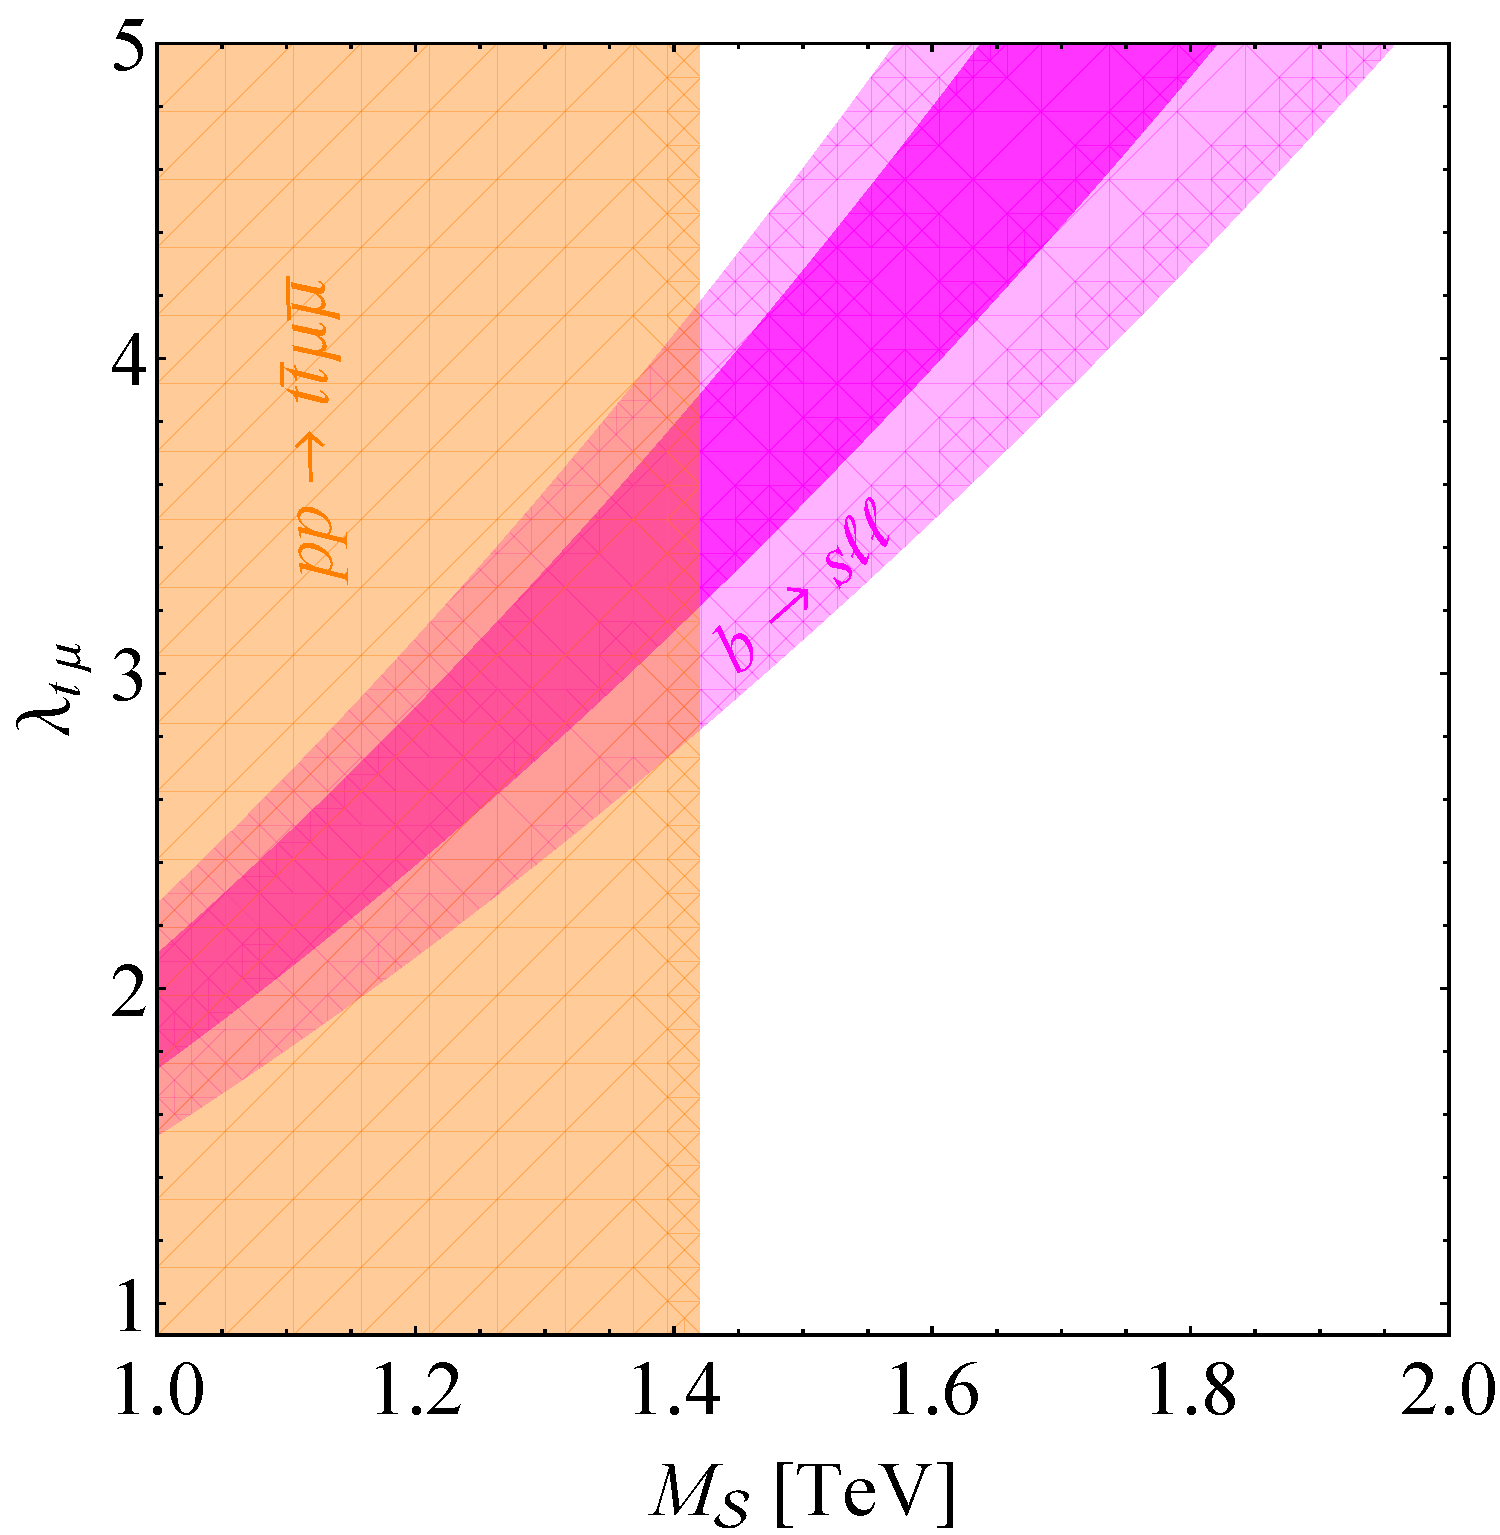
\includegraphics[width=0.45\linewidth]{figures/Scalar_LQ.pdf}
	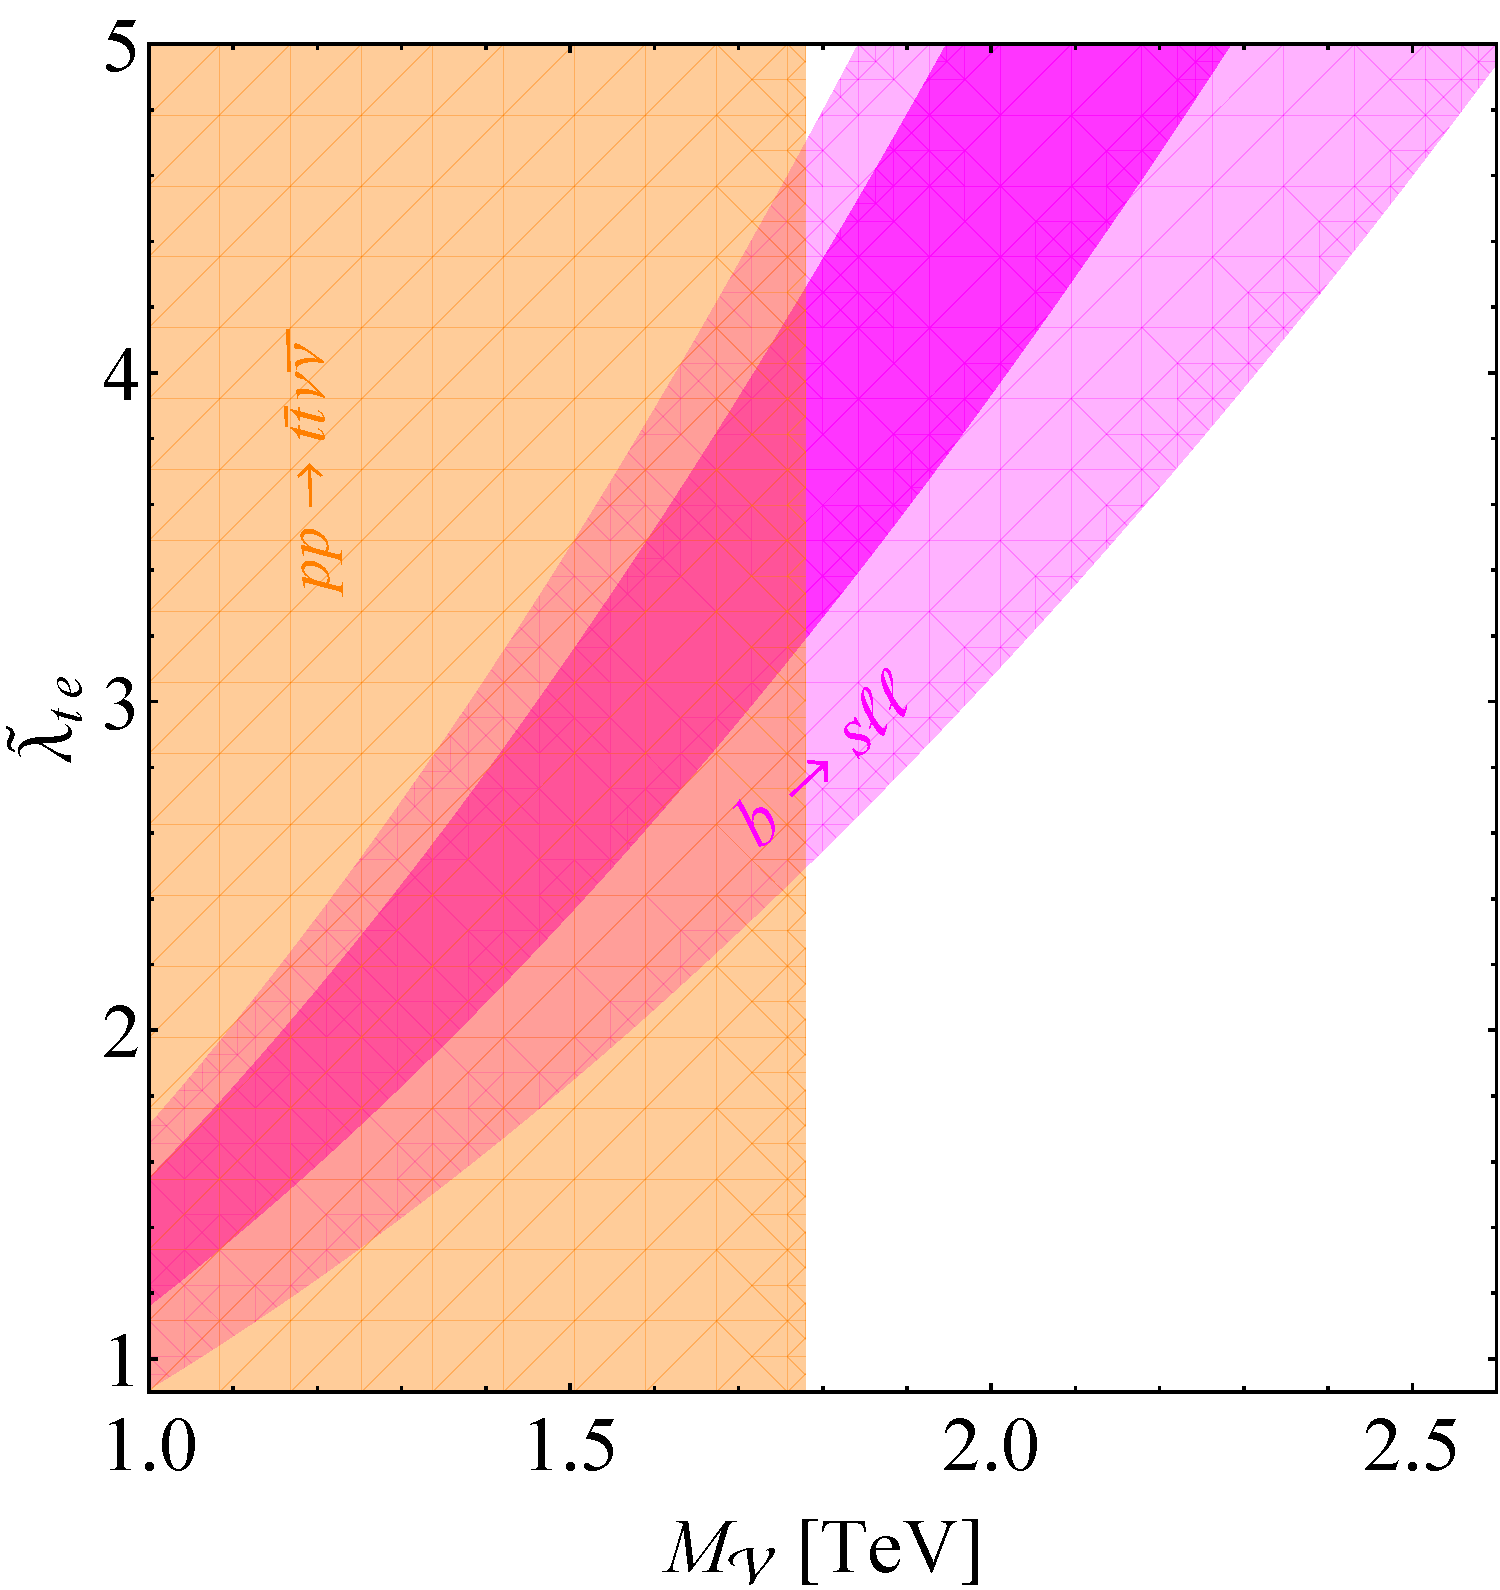
\includegraphics[width=0.435\linewidth]{figures/Vector_LQ.pdf}
	\caption{Constraints on the mass and LQ coupling with the muon for the scalar LQ model $\mathcal S$ on the left panel; while on the right panel the vector eletro-phillic LQ model parameters constraints are shown. The orange band shown the collider bounds based on comprehensive analysis found in ref.~\cite{Angelescu:2018tyl} The magenta regions show the models phase space at 68\% and 95\% CL that explains the flavour anomalies at one-loop.}    
	\label{fig:LQ_constraints}
\end{figure}
These leptoquarks can generate o $C_{\phi L}^{(1)}\ ^{\ell\ell}$ only at loop-level, see~\autoref{fig:genlqcphi}, which is insufficient to fulfil the requirements of the flavour + EWPO fit ~\autoref{fig:2D_correlations}. Hence, the addition of the extra singlet and triplet leptonic partners discussed in the previous section is again needed to survive EWPO constraints.
\begin{figure}[htpb!]
	\centering 
	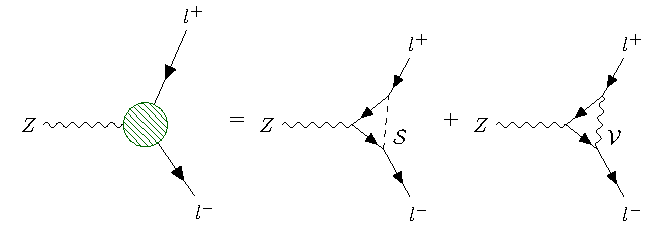
\includegraphics[width=\linewidth]{figures/LQ_tri}
	\caption{The leptoquarks considered can only generate  $C_{\phi L}^{(1)}\ ^{\ell\ell}$via loop matching. }    
	\label{fig:genlqcphi}
\end{figure}
%%%%%%%%%%%%%%%%%%
\section{Conclusion}
\label{sec:sum}
%%%%%%%%%%%%%%%%%%
This chapter addressed the $b \to s \ell \ell $ anomalies' resolution based on NP models that fall under the assumptions of MFV. Which required that LUV effects be generated at the loop level.  Moreover, the interplay between EWPO and these anomalies was portrayed in ~\autoref{fig:ew_flav_bounds} and, supported with \autoref{fig:ew_flav_dg}. \\

The global SMEFT fit performed hints that a unifying solution for EWPO and LUV anomalies can be achieved by including the right operators. Furthermore, the picture can be simplified by only having a minimum of $2$-$4$ SMEFT operators, portrayed in ~\autoref{fig:2D_correlations}. Like any multivariate analysis, the correlation amongst the coefficients played an essential role in finding the proper resolution of the EWPO and flavour observables conundrum. \\ 
Inspired by the simplified SMEFT model, we have discussed a top-phillic $Z^\prime$ model with top and muon vector-like partners. Moreover, an alternative, simpler model based on leptoquarks can also produce the $B$ anomalies at the loop level. Both models can be amended to include muonic or electronic solutions in the SMEFT simplified scenario. For the $Z^\prime$ model, the top and lepton partners need to have the same $X$ charge for the muon case, while they need to carry an opposite one for the electronic NP coupling.  The LQ models are different for the muonic and electronic; the former is compatible with scalar and the latter with vector LQs. \\ 

Both of these models required the inclusion of correlated pairs of vector-like leptons, a $SU(2)_L$ singlet and a triplet to realise the minimal EFT scenario depicted on~\autoref{fig:2D_correlations}. We observe that the existence of these particles may be independently motivated by the heavy new dynamics underlying the origin of neutrino masses and/or by a tentative explanation of the $(g-2)_{\mu}$ anomaly~\cite{Kannike:2011ng,Muong-2:2021ojo}.\\

Future measurements of $B$ decays by the LHCb and Belle-II are expected to reach a precision regime in the upcoming years ~\cite{Kou:2018nap,Bediaga:2018lhg}. These measurements, in addition to high-energy ones at linear colliders ~\cite{deBlas:2019rxi,deBlas:2019wgy} will reveal more about the nature of these anomalies and their connection with Higgs physics. This is already hinted at by the global fits done here with the current data predicting NP Higgs operators like $ C_{\phi L/e}$. Understanding how observables from different sectors correlate is essential to understanding the nature of NP underlying these anomalies, amongst others.


%We conclude by noting that the measurement of $B$ decays at the scale of a few GeV is expected to reach a precision regime with the completion of the future runs at LHC and SuperKEKB. Hence, better measurements of the LUV observables and angular distributions of $b\to s \ell \ell$ will be available in the next few years from Belle~II~\cite{Kou:2018nap} and LHCb~\cite{Bediaga:2018lhg}. These will add a fundamental verification of the current interpretation of $B$ anomalies and the direction in our search for NP signatures. 
%
%Along these lines, should these signals of LUV persist, their interplay with EW precision measurements could be further tested at future $e^+ e^-$ colliders. In particular, circular $e^+ e^-$ colliders running at the $Z$ pole, such as the FCC-ee~\cite{Abada:2019lih,Abada:2019zxq} or CEPC~\cite{CEPCStudyGroup:2018ghi}, could test deviations in the lepton universality of neutral weak currents with more than one order of magnitude improvement in precision compared to current data. At linear colliders, like the ILC~\cite{Bambade:2019fyw} or CLIC~\cite{deBlas:2018mhx}, where there is no proposed run at the $Z$ pole, it would still be possible to obtain a significant improvement in the measurements of EWPO via radiative return to the $Z$~\cite{Fujii:2019zll}. 
%
%Furthermore, the high-energy regime achievable at linear colliders would allow, after crossing the $t\bar{t}$ threshold, to directly test the effects of the interactions $O^{Lu,eu}_{1133}$ via $e^+ e^- \to t\bar{t}$. 
%For the muon case, on the other hand, to test $O^{Lu,eu}_{2233}$ one would still need to rely on more complicated signals, such as $t\bar{t}\mu^+\mu^-$, which would be, in any case, cleaner than at the LHC. (However, ideal optimal tests of these 4-fermion operators in 2-to-2 scattering processes require a high-energy muon collider.) All of these could represent valuable additions from a ``flavour'' perspective in the interpretation of EW (and Higgs) measurements at these future machines within the EFT framework~\cite{deBlas:2019rxi,deBlas:2019wgy}.

